\documentclass[binding=0.6cm, LaM]{sapthesis}
\usepackage{microtype}
\usepackage[english]{babel}
\usepackage[utf8]{inputenx}
\usepackage{hyperref}
\usepackage{wasysym}
\usepackage{siunitx}
\usepackage{biblatex}
\usepackage{titlesec}
\addbibresource{sample.bib}
\hypersetup{pdftitle={My thesis},pdfauthor={Giada Caneva Santoro}}
\usepackage{amsmath, amssymb}
\title{Building a template bank}
\author{Giada Caneva Santoro}
\IDnumber{1490713}
\course{Facolt\`a di Scienze Matematiche Fisiche e Naturali}
\courseorganizer{Corso di Laurea Magistrale in Fisica}
\AcademicYear{2018/2019}
\copyyear{2020}
\advisor{Dr. Francesco Pannarale Greco}
\authoremail{giada.greenday92@gmail.com}
\DeclareUnicodeCharacter{2212}{-}
\begin{document}

\frontmatter
\maketitle
\dedication{Fortsett å gå.}


\tableofcontents

\mainmatter 

\chapter{Introduction}

	More than 100 years ago, Albert Einstein predicted the existence of gravitational waves,
	GWs, on the basis of his theory of general relativity.  
	Einstein predicted that the motion of two bodies, such as planets or stars—orbit each other,
	could cause distortions of space-time, GWs \cite{1,2}, 
	These ripples in the fabric of space-time would spread out like the ripples in a pond when a stone is tossed in,
	although their amplitude would be so small that it would be nearly impossible to detect by any technology foreseen at that time.
	It was also predicted that objects moving in an orbit would lose energy for this reason 
	(a consequence of the law of conservation of energy), as some energy would be given off as GWs, 
	although this would be insignificantly small in all but the most extreme cases. 
	GWs squeeze and stretch anything in their path as they pass by. \\
	The most powerful GWs are created when objects move at very high speeds. 
	Examples of such things are orbiting pairs of black holes and neutron stars, 
	or massive stars blowing up at the ends of their lives.
	There are four categories of GWs based on what generates them: 
	continuous, compact binary inspiral, stochastic, and burst. 	
	Each category of objects generates a unique or characteristic set of signal 
	that LIGO-Virgo's interferometers can sense, and that researchers can look for in LIGO-Virgo’s data. \\ 
        The interferometers are designed to detect a specified range of frequencies of GWs,
        which means that they cannot detect objects orbiting at rates that fall outside of this range of frequencies 
        (either too low or too high). 
	During the final moments of the merger of two compact objects such as neutron stars 
	or black holes the emission of GWs is at its peak. The binary loses energy, 
	largely through GWs, and as a result, the two compact objects spiral in towards each other, 
	reaching extreme velocities at the very end of this process. 
	In the final fraction of a second of their merger a significant amount of their mass is converted into gravitational energy, 
	and travel outward as GWs, that potentially fall within the detector’s sensitive range. \\
	However, the time they spend orbiting in that range of frequencies is typically very brief.
        The masses of the objects involved dictate how long they emit detectable GWs. 
        Heavy objects, like black holes, move through their final inspiral phase much more rapidly than 'lighter' objects, 
        like neutron stars. This means that black-hole merger signals are much shorter than neutron star merger signals.
        For example, the first detection of a GW signal, GW150914, coming from the a pair of merging black holes, 
	produced a signal just two-tenths of a second long \cite{14}. 
        In contrast, the first neutron star merger LIGO detected in August 2017 generated a signal over 100 seconds long \cite{15}. \\
	This first observation was a a remarkable accomplishment: it demonstrated both the existence of binary stellar-mass black hole systems, 
	and the fact that such mergers could occur within the current age of the universe.  
	It also confirmed the last remaining unproven prediction of general relativity and validated 
	its predictions of space-time distortion in the context of large scale cosmic events. 
	Prior to this first detection, GWs had only been inferred indirectly,
        via their effect on the timing of pulsars in binary star systems.
	This event  marked the beginning of a new era of gravitational-wave astronomy, 
	which would enable observations of violent astrophysical events that were not previously possible, 
	and potentially allow the direct observation of the birth of the universe.


%----------------------------------------------------------------------------------------------------------------------------------------------------------------------------------------------------------
\chapter{Gravitational-Wave Detection Principles}

%warning: add a few lines to explain the chapter%

\section{Gravitational waves in linearized gravity}

	In 1915, Albert Einstein presented his general theory of relativity
	The classical Newtonian notion of gravity, which stated that gravity arises from an 
	action at a distance, was replaced by a geometric interpretation of the Universe, 
	the spacetime continuum: this may be regarded as a fabric and that can be curved 
	by mass \cite{1}. 
	The motion of masses on this curved spacetime fabric will then be perceived as gravity. 
	In general relativity, spacetime is regarded as a four-dimensional manifold 
	with a Lorentzian metric, and gravity is a manifestation of the manifold’s curvature. \\
	The spacetime curvature is associated with the stress-energy tensor 
	of matter fields through the Einstein field equation:
		\begin{equation}
		G_{\mu\nu} \equiv R_{\mu\nu}  - {1 \over 2}g_{\mu\nu}R = {8\pi G_{N} \over {c^4}}T_{\mu\nu} 
		\end{equation}
	where $G_{\mu\nu} $ is the Einstein tensor, $T_{\mu\nu} $ is the stress-energy 
	tensor of matter-fields and $ G_{N}$ is Newton’s gravitational constant. \\
	In 1916 Einstein found the weak-field solutions to general relativity had wave-like solutions, GWs.
	GWs are ripples in the fabric of spacetime, 
	which periodically lengthen and shorten space, and speed up and slow down time \cite{2}.
 	To study the properties of GWs, it is instructive to first study them 
	in situations where the gravitational fields are weak.
	In the so-called weak-field approximation, one can view the metric as the Minkowski metric 
	with a small perturbation: the Einstein equations can be expanded around the flat-space metric, of special relativity. \\
	Letting $ x_\mu = (t, x, y, z)$ denote the time and space coordinates, 
	we can write the proper distance between events $x_{\mu}$ and $x_{\mu} + dx_{\mu}$ as
		\[
		ds^2 = g_{\mu\nu}dx^{\mu}dx^{\nu} \approx (\eta_{\mu\nu} + h_{\mu\nu})dx_{\mu}dx_{\nu}. \hspace*{2cm}\|h_{\mu\nu}\|\ll 1
		\]
	Here $\eta_{\mu\nu} = diag(-1,1,1,1)$ is the usual Minkowski metric and the metric perturbation  $h_{\mu\nu}$         %decide if you want c and G% 
	represents the linearised gravitational field, it encapsulates GWs, 
	but contains additional, non-radiative degrees of freedom as well. $\|h_{\mu\nu}\|$ means
	“the magnitude of a typical non-zero component of $h_{\mu\nu}$”. 
	The condition $\|h_{\mu\nu}\|\ll 1$ requires both the gravitational field to be weak, 
	and constrains the coordinate system to be approximately Cartesian.  \\
	In linearized gravity, the smallness of the perturbation means that only terms which are linear in $h_{\mu\nu}$ are considered;
	higher order terms are discarded. As a consequence, indices are raised and lowered using the flat metric. 
	The metric perturbation $h_{\mu\nu}$ transforms as a tensor under Lorentz transformations, 
	but not under general coordinate transformations: since the numerical values of the components
	of a tensor depend on the reference frame, there exists a reference frame in which 
	the linearisation of the gravitational field holds on a sufficiently large region of the spacetime. \\
	The Einstein field equations are covariant under general coordinate transformations
		\begin{equation}
		x^{\mu} \rightarrow x^{\mu ‘}(x)
		\end{equation}
	So that the metric transforms as
		\begin{equation}
		g_{\mu\nu} \rightarrow g_{\mu' \nu'} = x^{\rho},_{\mu'}x^{\sigma},_{\nu'}g_{\rho \sigma}
		\end{equation}
	This means that one is free to choose a convenient coordinate system without 
	altering the physical predictions of the field equations \cite{16}. \\
	Choosing a reference frame breaks the invariance of general relativity under 
	coordiante trasformations but it also erases spurious degrees of freedom. 
	After choosing a frame where the field is linearised, 
	a residual gauge symmetry remains. \\
	Under infinitesimal coordinate transformations
                 \[
			x_{\mu} \rightarrow x_{\mu} + \xi_{\mu}
                \]
	using the transformation law of the metric, to lowest order $h_{\mu\nu}$ transforms as	
		\[
			h_{\mu\nu} \rightarrow h_{\mu\nu} - \partial_{\mu}\xi_{\nu} - \partial_{\nu}\xi_{\mu}
		\]
	Rather than working with the metric perturbation, changing notation and using the trace-reversed perturbation 
	makes the computation more compact and cleaner. We define
		\begin{equation}
			{\bar h}_{\mu\nu} = h_{\mu\nu} - {1 \over {2}}\eta_{\mu\nu}h  
		\end{equation}
	the trace
		\begin{equation}
			h = \eta^{\mu\nu}h_{\mu\nu}
		\end{equation}
	and express the trace-reversed field:
		\begin{equation}
			h_{\mu\nu} = {\bar h}_{\mu\nu} + {1 \over {2}}\eta_{\mu\nu}{\bar h}
		\end{equation}
	The Rienmann tensor constructed in the linearised theory is given by
		\begin{align}
			R^{\mu}_{\nu\rho\sigma} &= \partial_{\rho} \Gamma^{\mu}_{\nu\sigma} - \partial_{\sigma}\Gamma^{\mu}_{\nu\rho}  \\
				       &= {1 \over 2} (\partial_{\rho}\partial_{\nu}h^{\mu}_{\nu\rho} + \partial_{\sigma}\partial^{\mu}h^{\nu\rho} - \partial_{\rho}\partial^{\mu}h^{\nu\sigma} - \partial_{\					     \sigma}\partial_{\nu}h^{\mu}_{\rho})
		\end{align}
	From this, the Ricci tensor takes the form
		\begin{equation}
			R_{\mu\nu} = R^{\rho}_{\mu\rho\nu} = {1 \over 2}(\partial_{\rho}\partial_{\nu}h^{\rho}_{\mu} + \partial^{\rho}\partial_{\mu}h_{\nu\rho} - \square h_{\mu\nu} - \partial_{\mu}\partial_{\nu}h)
		\end{equation}
	The curvature scalar is obtained contracting once more:
		\begin{equation}
			R = R^{\mu}_{\mu} = (\partial_{\rho}\partial^{\mu}h^{\rho}_{\mu} - \square h)
		\end{equation}
	Finally, the Einstein tensor can be expressed as
		\begin{equation}
			G_{\mu\nu} = {1 \over 2}(\partial_{\rho}\partial_{\nu}h^{\rho}_{\mu} + \partial^{\rho}\partial_{\mu}h_{\nu\rho} - \square h_{\mu\nu} - \partial_{\mu}\partial_{\nu}h - \eta_{\mu\nu}\partial_{\rho}\partial^{\sigma}h^{\rho}_{\sigma} + \eta_{\mu\nu}\square h)
		\end{equation}
	Substituting the metric perturbation $h_{\mu\nu}$  with the $trace-reversed$ perturbation ${\bar h}_{\mu\nu}$ and expanding, 
	the linerised Einstein equations take the compact form:
		\begin{equation}
			\square {\bar h}_{\mu\nu} + \eta_{\mu\nu}{\partial}^{\rho}{\partial}^{\sigma}{\bar h}_{\rho\sigma} - {\partial}^{\rho}{\partial}^{\nu}{\bar h}_{\mu\rho} - {\partial}^{\rho}{\partial}^{\mu}{\bar h}_{\nu\rho} = - {{16\pi G_{N}} \over {c^4}}T_{\mu\nu}.
		\end{equation}
	The linearised equations of motion are gauge-invariant, and the gauge freedom can
 	be used to simplify the form of the field equations \cite{17}.
 	In the Lorentz family of gauges, choosing the harmonic gauge $ \partial_{\mu}h_{\mu\nu} = 0 $ 
	reduces the Einstein equations to a simple wave equation that relates the trace-reversed field
 	to the stress energy tensor:
		\begin{equation}
			\label{reduceinstein}
			\square {\bar h}_{\mu\nu} =({\partial^2 \over {\partial t^2} } - {\partial^2 \over {\partial x^2}}  - {\partial^2 \over {\partial y^2}}  -  {\partial^2 \over {\partial z^2}}) {\bar h}_{\mu\nu} = -{{16\pi G_{N}} \over {c^4}}T_{\mu\nu}. 
		\end{equation}
	By imposing the harmonic gauge one has chosen the coordinates in such a way that for a single plane wave 
	(or a superposition of plane waves with their wave vectors pointing in the same direction),
	the GW polarisations are perpendicular to the direction of propagation.
	The harmonic gauge gives four conditions, that reduce the ten indipendent components of  
	$h_{\mu\nu}$ to six indipendent components, so it does not fix the gauge completely,
	leaving four additional components free to be gauge-fixed.
	If the metric perturbation is not in the harmonic gauge, by making an infinitesimal coordinate transformation
		\begin{equation}
			{\bar h}_{\mu\nu} \rightarrow {\bar h}_{\mu’\nu’}  = {\bar h}_{\mu\nu}  - \xi_{\mu,\nu} -\xi_{\nu,\mu} + \eta_{\mu\nu}\xi^{\rho}_{,\rho}
		\end{equation}
	and applying the harmonic gauge condition
		\begin{equation}
			{\bar h}_{\mu’\nu’,} ^{\nu’} = {\bar h}_{\mu\nu,} ^{\nu} - \xi_{\mu,\nu}^{\nu}
		\end{equation}
	Therefore any metric perturbation can be put into an harmonic gauge by making an infinitesimal 
	coordinate transformation that satisfies
		\begin{equation}
			{\bar h}_{\mu\nu,} ^{\nu} = \xi_{\mu,\nu}^{\nu}
		\end{equation}
	This is a wave equation that always admits a solution, thus one can always achieve the harmonic gauge. 
	Outside the source where $T_{\mu\nu} = 0$ Eq.$\ref{reduceinstein}$ reads 
		\begin{equation}
			\square {\bar h}_{\mu\nu} = 0
		\end{equation}
	In asymptotically flat ($h_{\mu\nu} \rightarrow 0$ as $r \rightarrow 0$) vacuum spacetimes, 
	the metric perturbation can be greatly simplified using
	the residual gauge freedom within the harmonic gauge class \cite{4}. 
	The transverse-traceless $TT$-gauge can be obtained by choosing the components of the metric tensor $h_{\mu\nu}$
	so that only the ones on the plane orthogonal to the direction of propagation (transverse) 
	are different from zero; this results in $h_{\mu\nu}$ being traceless:
		\begin{equation}
			h^{0\mu} = 0 \hspace*{0.5cm}  h^{i}_i = 0  \hspace*{0.5cm}   {\partial}^jh_{ij} = 0
		\end{equation}
	By imposing the harmonic gauge, the ten degrees of freedom of $h_{\mu\nu}$ 
	have reduced to six degrees of freedom, and the residual gauge freedom,
	associated to the four functions $\xi^{\mu}$, has further reduced these to just two degrees of freedom, 
	which correspond to the two possible polarization states of the GW. 
	Equation (2.17) has plane wave solutions $h_{\mu\nu}^{TT}(x)=e_{ij}(k)e^{ikx}$ with 
	$k^{\mu}=(\omega/c,k)$ and $\omega/c=|k|$. The tensor $e_{ij}(k)$ is called the polarization tensor. \\
	In vacuum spacetimes, a plane GW with a given wave-vector $k$ is characterized 
	by two functions $h_+$ and $h_{\times}$, while the remaining components can be set to zero by
	choosing the transverse-traceless gauge. 
	Along the z axis:
		\begin{equation} 
		h_{\mu\nu}^{TT} = 
		\begin{bmatrix}
		0 & 0 & 0 & 0 \\
		0 & h_{+} & h_{\times} & 0 \\
		0 & h_{\times} & -h_{+} & 0 \\
		0 & 0 & 0 & 0 
		\end{bmatrix}\cos{\omega(t-z/c)}
		\end{equation}

\subsubsection{Geodesic equation and geodesic deviation}

	The usual notion of “gravitational force” disappears in general relativity, replaced instead 
	by the idea that freely falling bodies follow geodesics in spacetime.
	Geodesics are the curved-spacetime equivalents of straight lines, which can be found by 
	parallel transporting the tangent vector of a curve \cite{16}. \\
	Given a spacetime metric $g_{\mu\nu}$ and a set of spacetime coordinates $x^{\mu}$, 
	geodesic trajectories are given by the equation:
		\begin{equation}
			{{d^2x^{\mu}}\over{d\tau^2}} + \Gamma_{\nu\rho}^{\mu}(x){{dx^{\nu}}\over{d\tau}}{{dx^{\rho}}\over{d\tau}} = 0 \hspace*{2cm} m \neq 0
		\end{equation}
		\begin{equation}
			{{d^2x^{\mu}}\over{d\lambda^2}} + \Gamma_{\nu\rho}^{\mu}(x){{dx^{\nu}}\over{d\lambda}}{{dx^{\rho}}\over{d\lambda}} = 0 \hspace*{2cm} m = 0
		\end{equation}
	which is the classical equation of motion of a test mass in the curved background described 
	by the metric $g_{\mu\nu}$, in the absence of an external non-gravitational force and where $m$ is the mass
	of the object, $\tau$ represents the proper time given by $d\tau^2 = -ds^2$, 
	and $\lambda$ is some affine parameter along the geodesic. \\
	In a flat spacetime, two straight lines that are initially parallel to each other will remain parallel. \\
	In a curved spacetime, geodesics do not satisfy this property.
	Instead, two nearby geodesics, separeted by $\zeta^{\mu}$, follow the geodesic deviation equation
		\begin{equation}
			{{D^2\zeta^{\mu}}\over{D\tau^2}} = -R^{\mu}_{\nu\rho\sigma}\zeta^{\rho}{{dx^{\nu}}\over{d\tau}}{{dx^{\sigma}}\over{d\tau}}
		\end{equation}
	where $D/D\tau$ is defined as
		\begin{equation}
			{{DV^{\mu}}\over{D\tau}} \equiv {{dV^{\mu}}\over{d\tau}} + \Gamma^{\mu}_{\nu\rho}V^{\nu}{{dx^{\rho}}\over{d\tau}}
		\end{equation}
	and denotes the covariant derivative along a curve parameterised by $\tau$. 
	The geodesics deviation equation describes the change in separation $\zeta^{\mu}$ between two nearby geodesic. \\
	As the Rienmann tensor describes the tidal forces caused by the gravitational field, 
	the geodesic deviation equation shows that tidal forces can be considered as deviations of nearby geodesics \cite{6}.

%----------------------------------------------------------------------------------------------------------------------------------------------------------------------------------------------------------
\section{Gravitational wave detection with laser interferometers}

	Electromagnetic waves interact strongly with matter, while GWs travel unperturbed through space,
        as they interact only very weakly with matter. This makes them an excellent probe for astrophysicalphenomena that dark
        in the electromagnetic channel, such as the coalescence and merger of black holes, the collapse of a stellar core,
  	the dynamics of the early Universe. However, it also means that detecting GWs is extremely challenging.
        Electromagnetic radiation typically has a wavelength smaller than the size of the emitting system,
        and so can be used to form an image of the source, while the wavelength of gravitational radiation is typically comparable
        to or larger than the size of the radiating source \cite{18}. \\
        Because GWs are generated by the bulk dynamics of the source itself therefore they cannot be used to form an image:
        the radiation simply does not resolve the generating system.
        In most cases, electromagnetic astronomy is based on observers obtain a large amount of information about sources on a small piece
        of the sky while GW astronomy is intrinsically an all-sky approach \cite{4}. \\
	The experimental search for GWs was initiated by Joseph Weber in the early 60  \cite{7}.
	Weber’s first GW detector was a resonant bar detector; 
	the detection’s principle behind these instruments is that 
	they would be set into oscillation at their resonant frequency 
	by passing GWs near that resonant frequency.
	For this purpose, Weber designed and built a big aluminum cylinder as a sort of antenna, 
	hung by a steel wire from a support to isolate vibrations of its environment. 
	The whole instrument was placed inside a vacuum chamber 
	and the cylinder surrounded by a belt of piezoelectric crystal, 
	to sense cylinder vibrations induced by GWs.
	Even though, over the course of the following years, the bar detectors’ sensitivity increased, 
	it did not reach a level where they would be able to detect an extragalactic source. \\
	The first explicit suggestion of a laser interferometer detector 
	was outlined by Gertsenshtein and Pustovoid in 1962 \cite{8}. \\
	From the early 2000s, several kilometer-scale ground-based interferometers 
	operated in the frequency band from $10 Hz$ to $1 kHz$ at a sensitivity 
	that all owed the potential for detection from a variety 
	of sources at large extragalactic distances.

\subsection{Description of laser interferometers}

	The optical layout of the detectors consists in perpendicular 
	Fabry–Perot arm cavities of the Michelson, 
	with lasers running along the 4 km arms, as shown in Fig.$\ref{fig:interferometer}$. 
	A beam splitter directs 1064 nm light from a diode-pumped, power amplified, 
	and intensity and frequency stabilized Nd:YAG laser to the Fabry-Perot arms, 
	which are made of an input test mass mirror and an end test mass mirror. 
	The two beams of laser light that return from the two arms are recombined out of phase so that, 
	in principle, no light reaches the so-called 'dark fringe' of the detector. 
	The oscillating quadrupolar strain pattern of a GW, 
	as seen in Fig.$\ref{fig:ring}$, is well matched by a Michelson interferometer,
        which makes a very sensitive comparison of the lengths of its two orthogonal arms.
	Any variation caused by an alteration in the distance between the mirrors, 
	produces a very small shift in phase between the beams and, thus, 
	a variation of the intensity of the light, which is proportional to the wave's amplitude. \cite{10}. \\
	The Fabry-Perot arms are a modification to the Michelson 
	that increases the change in phase measured compared to that for a simple Michelson: 
	because of multiple reflections that occur within each cavity, 
	the tiny distance variation caused by a GW is amplified. \\
	All the main interferometer optical components and beam paths are enclosed in the ultra-high vacuum system
        $(10^{−8} - 10^{−9} torr)$ for acoustical isolation and to reduce phase fluctuations from light scattering off residual gas.
        The photodetectors are all located outside the vacuum system, mounted on optical tables.
        The beam tubes are made from stainless steel and are designed to have low-outgassing
        so that the required vacuum can be attained by pumping only from the ends of the tubes \cite{11}. \\
        The interferometer optics, including the test masses, are manufactured to have extremely low scatter and low absorption.
	The GW detectors offer the possibility of very high sensitivities over a wide range of frequency and
        are particularly suited for the detection of local perturbations in the spacetime metric from astrophysical sources,
        such as binary black hole or neutron star coalescences, asymmetric rapidly spinning neutron stars,
        and supernovae . \\
 	Gravitational radiation is produced by oscillating multipole moments of the mass distribution of a system.
        Quadrupole radiation is the lowest allowed form, and is thus usually the dominant form.
        In this case, the GW field strength is proportional to the second time derivative of the quadrupole moment of the source,
        and it falls off in amplitude $h$, the direct observable of gravitational radiation, with distance as $1/r$.
        This comparatively slow fall off with distances means that relatively small improvements in the sensitivity
        of GW detectors can have a large impact on their science:
        doubling the sensitivity of a detector doubles the distance to which sources can be detected,
        increasing the volume of the Universe to which sources are measurable by a factor eight. \\
	The frequency band $1Hz \apprle f \apprle 10^4 Hz$ is targeted by
        ground-based laser interferometric detectors has its low end set by the fact that it is extremely difficult
        to prevent mechanical coupling of the detector to ground vibrations at low frequencies,
        and probably impossible to prevent gravitational coupling to ground vibrations, human activity, and atmospheric motions.
    \begin{figure}
                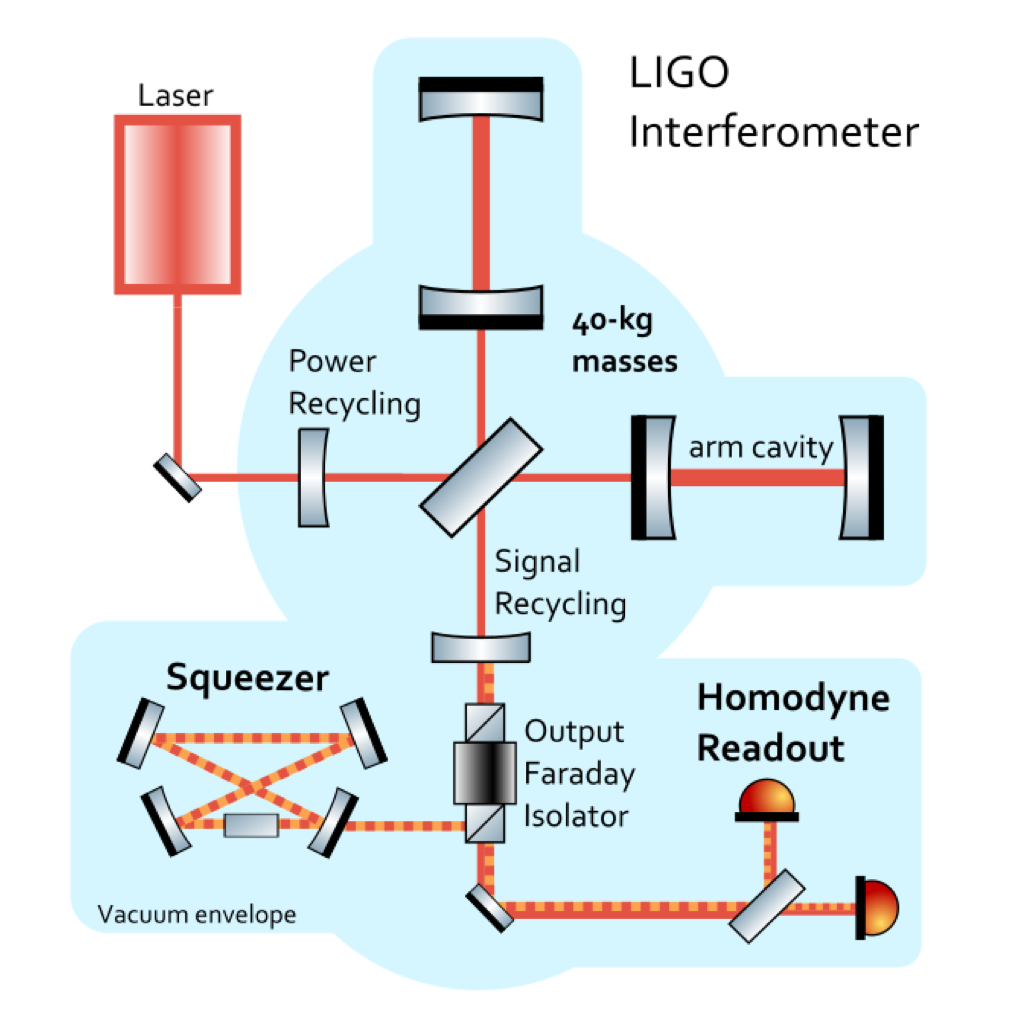
\includegraphics[scale=0.5]{interferometer}
                \centering
                \caption{Simplified schematic of the experimental setup.  
			 Several modifications to the Michelson interferometer 
			 are shown such as power and signal recycling. 
			 The photodetector records the differential lengths of the arms. \cite{9}}
                \label{fig:interferometer}
                \end{figure}

\subsection{Ground-based laser interferometers}

	Detectors have nearly $4\pi$ steradian sensitivity to events over the sky. 
	This means that any source on the sky will be detectable,
        not just sources in specific pointing directions. \\
	A single interferometer is unable to detect GW alone,
	because it us difficult to separate a signal from noise confidently 
	and also provides no directional information about the source.
	A worldwide network of detector is essential to a successful GW detection:
	looking for identical, simultaneous signals from multiple detectors worldwide, 
	rules out noise sources which are local to a given detector. 
	More detectors means a better determination of the direction of GW sources: 
	to reconstruct the location of a transient signal is primarily due to triangulation 
	based on the observed time delays of the signal at several detectors. 
	For more than two sites, requiring a consistency between the observed amplitudes 
	will also serve to restrict the allowed sky positions\cite{12}. \\
	A crucial aspect of the research is to make the instrument sufficiently sensitive:
        at the targeted strain sensitivity of $10^{−21}$ m, the resulting arm length change is only $ 10^{-18}$ m for km-scale instruments, that is
        a thousand times smaller than the diameter of a proton.
        A key feature of the detectors is simply their scale:
        the arms are made as long as practically possible to increase the signal due to a GW strain. \\
	We now briefly list current GW interferometers.

	\begin{itemize}
		\item LIGO. LIGO operates two identical and far apart GW observatories: 
			    LIGO Hanford, in Washington, and LIGO Livingston, in Louisiana.
			    The sites are separated by roughly 3000 km, 
		   	    and are situated to support coincidence analysis of events.
		       	    LIGO's original instrument engaged in "science observations" from 2002 to 2010. 
			    During this initial phase, the Hanford site operated two collocated interferometers:
			    one detector with 4 km long arms (H1) and another with 2 km long arms (H2). 
			    The Livingston site operated a second 4 km detector (L1). 
			    Each observatory is made up of ultra high vacuum system, 
			    where the interferometer is placed. \\
			    This Advanced LIGO project successfully improved the capabilities of the detectors, 
			    both interferometers were completely overhauled to incorporate much more sophisticated engineering.
		\item Virgo. The Advanced Virgo detector, located in Cascina (near Pisa) in Italy, 
			     is the upgraded version of the Virgo detector. 
			     As LIGO, it is a Michelson interferometer but with 3 km arms.
                 \item GEO600. GEO600 is a 600 m interferometer located near Hannover,
                 	       Germany. It is designed and operated by scientists from the
                               Max Planck Institute for Gravitational Physics and the Leibniz Universität Hannover.
                  \item KAGRA. It is Japan’s first GW detector and also the first GW detector to operate
			       at cryogenic temperatures, improving sensitivity at frequencies around 100 Hz.

\end{itemize}

\section{Interaction of gravitational waves with test masses}
	
	The effects of GWs cannot be seen in isolated bodies. 
	This is a result of the fact that a single test mass, 
	in a frame freely falling with it, will remain at rest.
	At least two test masses are required to measure the effects of GWs. 	
	This is also the case when one wants to measure any curvature of spacetime. \\
        Therefore, to understand how GWs interact with the interferometric detectors,
        it is necessary to use the geodesic equation and the geodesic deviation equation, which are also important tools
        for understanding the physical meaning of a given gauge choice \cite{3}. 
        In fact the physics must be invariant under coordinate trasformations but GWs and the detector description's depend on the chosen reference frame.
        Consider a test mass initially at rest at $\tau = 0$. \\
	The geodesic equation then becomes
                \begin{equation}
                	{{dx^i}\over{d\tau^2}} = -[\Gamma^i_{\nu\rho}{{dx^{\nu}}\over{d\tau}}{{dx^{\rho}}\over{d\tau}}]_{\tau=0} \\ 
                			       = - [ \Gamma^i_{00}({{dx^0}\over{d\tau}})^2]_{\tau=0}
                \end{equation}
        because
                \begin{equation}
                	{{dx^i}\over{d\tau}} = 0 \hspace*{2cm} at \hspace*{0.5cm}\tau = 0
                \end{equation}
        since the mass is initially at rest. Expanding to first order in $h_{\mu\nu}$,
        the Christoffel symbol $\Gamma^i_{00} = 1/2(2\partial_{0}h_{0i} - \partial_i h_{00})$ vanishes in the TT gauge
        because both $h_{00}$ and $h_{0i}$ are set to zero by the gauge condition. \\
        Therefore, if at time $\tau = 0$ $dx^i/d\tau$ is zero, it remains zero at all times,
        because its derivative also vanishes.
        This shows that if two test masses are initially separated by a coordinate separation of $x^i$ in the TT frame,
        and are at rest with respect to each other, they will remain at this separation.
        Overall, it seems that a GW has no influence on the geodesic or on the deviation of geodesics. 
        In other words, in the TT gauge the coordinate location of a slowly moving, free-falling body is unaffected
        by a GW because the coordinates move with the waves \cite{4}. \\
        The TT gauge illustrates that, in general relativity, the physical effects are not expressed by what happens
        to the coordinates since the theory is invariant under coordinate transformations:
        the position of test masses does not change because the gauge freedom allowed to define the coordinates
        in such a way that they do not change \cite{3}.
        Physical effects can instead be found monitoring proper distances, or proper times. 
        GWs cause the proper separation between two freely falling particles to oscillate,
        even if their coordinate separation is constant. Consider two  free-falling particles,
        located at $z = 0$, and separated on the $x$ axis by a coordinate distance $L_c$. \\
        Consider a GW in TT gauge that propagates down the $z$ axis, $h^{TT}_{\mu\nu}(t,z)$.
        The proper distance L between the two particles in the presence of the GW is given by
                \begin{align}
                \label{distance}
                	L & = \int^{L_c}_{0}{dx\sqrt{g_{xx}}} = \int^{L_c}_{0}dx\sqrt{1 + h^{TT}_{xx}(t,z=0)} \\
                	  & \simeq \int^{L_c}_{0}{dx[1 + {1 \over 2}h^{TT}_{xx}(t,z=0)]} \\
                	  &= L_c[1 + {1 \over 2}h^{TT}_{xx}(t,z=0)]
                \end{align}
        Therefore, the proper distance expands and shrinks periodically, with a fractional length change $\delta L/L_c$ given by
                \begin{equation}
                	{{\delta L}\over{L_c}} \simeq {1 \over 2} h_{xx}^{TT}(t,z=0)
                \end{equation}
        Even though this result is calculated in the TT gauge, it is indeed gauge indipendent;
        $h_{xx}^{TT}$ acts as a strain, a fractional length change.
        Because the time that light travels between the two test masses is related to the proper distance,
        which directly relates to the accumulated phase measured by laser interferometric GW observatories,
        GWs leave an imprint on the time it takes for a photon to make a round trip \cite{4}. \\
        Consequently, interferometers can potentially measure these imprints by measuring the length difference between
        their arms. The “extra” phase $\delta \phi$ (if $L \ll \lambda$ so that the metric perturbation
	does not vary during a light travel time) accumulated by a photon that travels
        down and back the arm of a laser interferometer in the presence of a GW is $\delta \phi = 4\pi \delta L \lambda$,
        where $\lambda$ is the photon’s wavelength and $\delta L$ is the distance
        the end mirror moves relative to the beam splitter.

\subsection{Local proper reference frame}

        Since positions in a lab are not marked by test particles,
        the $TT$ frame is not very practical.
        The preferred reference frame is the proper detector frame
        in which the test particle is free to move because of a passing GW.
        The path of a test particle can then be described by Newtonian equations of motion in terms of forces.
        There are terms proportional to the Riemann curvature tensor from the gravitational field of the Earth
        but also terms from static gravitational forces, Coriolis forces, etc \cite{5}.
	GW detectors need to be designed in order to maximise their sensitivity to the part proportional to the Riemann tensor while minimizing their sensitivity to all other terms.
        Consider a detector capable of measuring changes in the proper distance, between two test masses
        and assume the detector has a characteristic size that is much smaller
        than the characteristic wavelength of the GW. \\
        In this case, one can approximate the entire detector to be in a near local Lorentz frame
        (freely falling frame), even in the presence of GWs. This coordinate system is defined by the requirements
                \begin{equation}
                	z^i(\tau) = 0, \hspace*{2cm} g_{ab}(t, 0) = \eta_{ab}, \hspace*{2cm} \Gamma^a_{bc}(t,0) = 0,
                \end{equation}
        which imply that the metric has the form
                \begin{equation}
                	ds^2 \approx -dt^2 + \delta_{ij}dx^i dx^j + O({{x^ix^j}\over{L^2_B}})
                \end{equation}
        where $L^2_B$ denotes the typical variation scale of the metric. \\
        Consider now the proper distance between the two geodesics of the test masses, $\zeta^i$.
        The GWs influence these two test masses via the geodesic deviation equation
                \begin{equation}
                	{{d^2\zeta^{\mu}}\over{d\tau^2}} + 2\Gamma^{\mu}_{\nu\rho}{{dx^{\nu}}\over{d\tau}}{{dx^\rho}\over{d\tau}} + \zeta^{\sigma}\Gamma^{\mu}_{\nu\rho,\sigma}{{dx^{\nu}}\over{d\tau}}{{dx^{\rho}}\over{d\tau}} = 0
                \end{equation}
        Assuming the two test masses are moving non-relativistically, $dx^i/d\tau$ can be neglected compared to $dx^0/d\tau$. \\
        Furthermore, the term proportional to $\Gamma^{\mu}_{\nu\rho}$ is negligible compared to other terms in a near  local-Lorentz frame, LLF. Hence,
                \begin{equation}
                	{{d^2\zeta^{\mu}}\over{d\tau^2}} + \zeta^{\sigma}\Gamma^{i}_{00, \sigma}({{dx^0}\over{d\tau}})^2 = 0
                \end{equation}
        Further simplifying $\zeta^{\sigma}\Gamma^{i}_{00, \sigma} \approx \zeta^{j}\Gamma^{i}_{00, j}$
                \begin{equation}
                	{{d^2\zeta^{\mu}}\over{d\tau^2}} + \zeta^{j}\Gamma^{i}_{00,j}({{dx^0}\over{d\tau}})^2 = 0
                \end{equation}
        But in the LLF, $R^i_{0j0} = \Gamma^i_{00,j} - \Gamma^i_{0j,0} = \Gamma^i_{00,j}$ and therefore
                \begin{equation}
                	{{d^2\zeta^{\mu}}\over{d\tau^2}} + R^i_{0j0} \zeta^j({{dx^0}\over{d\tau}})^2 = 0
                \end{equation}
        Because $dx^0/d\tau \approx 1$, one can approximate $\tau \approx t$:
                \begin{equation}
                	{\ddot \zeta}^j = - R^i_{0j0}\zeta^j
                \end{equation}
        The key quantity entering into the equation, the Rienmann tensor, is gauge invariant in the linearized theory and
        it can be evaluated in any convenient coordinate system. \\
        The expression for the Rienmann tensor in terms of the TT gauge metric perturbation $h_{ij}^{TT}$ is
                \begin{equation}
                	R^i_{0j0} = R_{i0j0} = - {1 \over 2}{\ddot h}_{ij}^{TT}
                \end{equation}
        Substituting into the previous equation, the geodesic deviation equation in the proper detector frame takes the form
                \begin{equation}
                	{\ddot \zeta}^i = {1 \over 2}{\ddot h}_{ij}^{TT}\zeta^j
                \end{equation}
        which can be interpreted as if the influence of a GW in a near LLF resembles a Newtonian force. \\
        Generalizing Eq.$\ref{distance}$, the proper distance may be written as
                \begin{equation}
                	s = \sqrt{L^2 + h_{ij}(t)L_{i}L_{j}}
                \end{equation}
        where $L_i$ denotes the spatial separation between two test masses and $L$ the associated coordinate distance.
        In the given metric for the proper reference frame, the proper distance is just $|L| = \sqrt{L_iL_j}$ up to fractional errors;
        since we are considering detectors such that
        $L \ll \lambda$, these errors are smaller than the fractional distance changes caused by the GW. \\
        Therefore $|L|$ is simply identified as the proper separation. The equation for analyzing an interferometric GW detector is therefore
                \begin{equation}
                	{\ddot L}^i = {1 \over 2}{\ddot h}_{ij}^{TT}L^j
                \end{equation}

\subsection{Ring of test masses}

        Consider a ring of test masses in the $(x, y)$ plane of a proper detector frame, initially at rest, centred at $z = 0$,
        and a GW travelling in the $z$-direction.
        This situation restricts the attention to the $(x,y)$ plane alone, because $h_{ij}^{TT}$ is transverse to the propagation direction,
        so the GW will only have influence in the plane of the test masses:
        the only non zero compontents of the metric perturbation are
                \begin{equation}
                	h_{xx}^{TT} = - h_{yy}^{TT} = h_{+} \hspace*{3cm} h_{xy}^{TT} = h_{yx}^{TT} = h_{\times}
                \end{equation}
        where $h_{+}=h_{+}(t-z)$ and $h_{\times}=h_{\times}(t-z)$ are the two polarization components, which are indipendent and can be considered separately.
        For the plus polarization at $z=0$ and initial conditions $h_{ij}^{TT} = 0$ at $t=0$:
                \begin{equation}
                h_{ab}^{TT} = 
                \begin{bmatrix}
                1  & 0 \\
                0 &  -1 \\
                \end{bmatrix} 
                h_{+}\cos \omega t
                \end{equation}
        If the displacement between geodesics is $\zeta_a (t) = (x_0 + \delta x(t), y_0 + \delta y(t))$, then
                \begin{equation}
                	\delta {\ddot x} = - {{h_{+}} \over 2} (x_0 + \delta x) \omega ^2 \sin \omega t
                \end{equation}
                \begin{equation}
                	\delta {\ddot y} =  {{h_{+}} \over 2} (y_0 + \delta y) \omega ^2 \sin \omega t
                \end{equation}
        Assuming that the perturbations are $O(h)$, and thus small compared to the unperturbed locations, $\delta x$ and $\delta y$ can be neglected.
        The integrations gives the deviations caused by the plus polarisations:
                \begin{equation}
                	\delta x(t) =  {{h_{+}} \over 2} x_0 \sin \omega t
                \end{equation}
                \begin{equation}
                	\delta y(t) = - {{h_{+}} \over 2} y_0  \sin \omega t
                \end{equation}
        Similarly, for the cross polarization at $z=0$ and initial conditions $h_{ii}^{TT} = 0$ at $t= 0$, the situation is described by the equations
                \begin{equation}
                	\delta x(t) =  {{h_{\times}} \over 2} y_0 \sin \omega t
                \end{equation}
                \begin{equation}
                	\delta y(t) =  {{h_{\times}} \over 2} x_0  \sin \omega t
                \end{equation}
        This set of equations describes the changes in the $x$ and $y$ components for a passing GW.
        The plus polarization alternately stretches and compresses the ring of test masses in the x and y directions,
        while the cross polarization exhibits the same behavior rotated by $\ang{45}$ in the $x - y$ plane. This is shown in Figure 2.1.
                \begin{figure}
                \label{ring}
                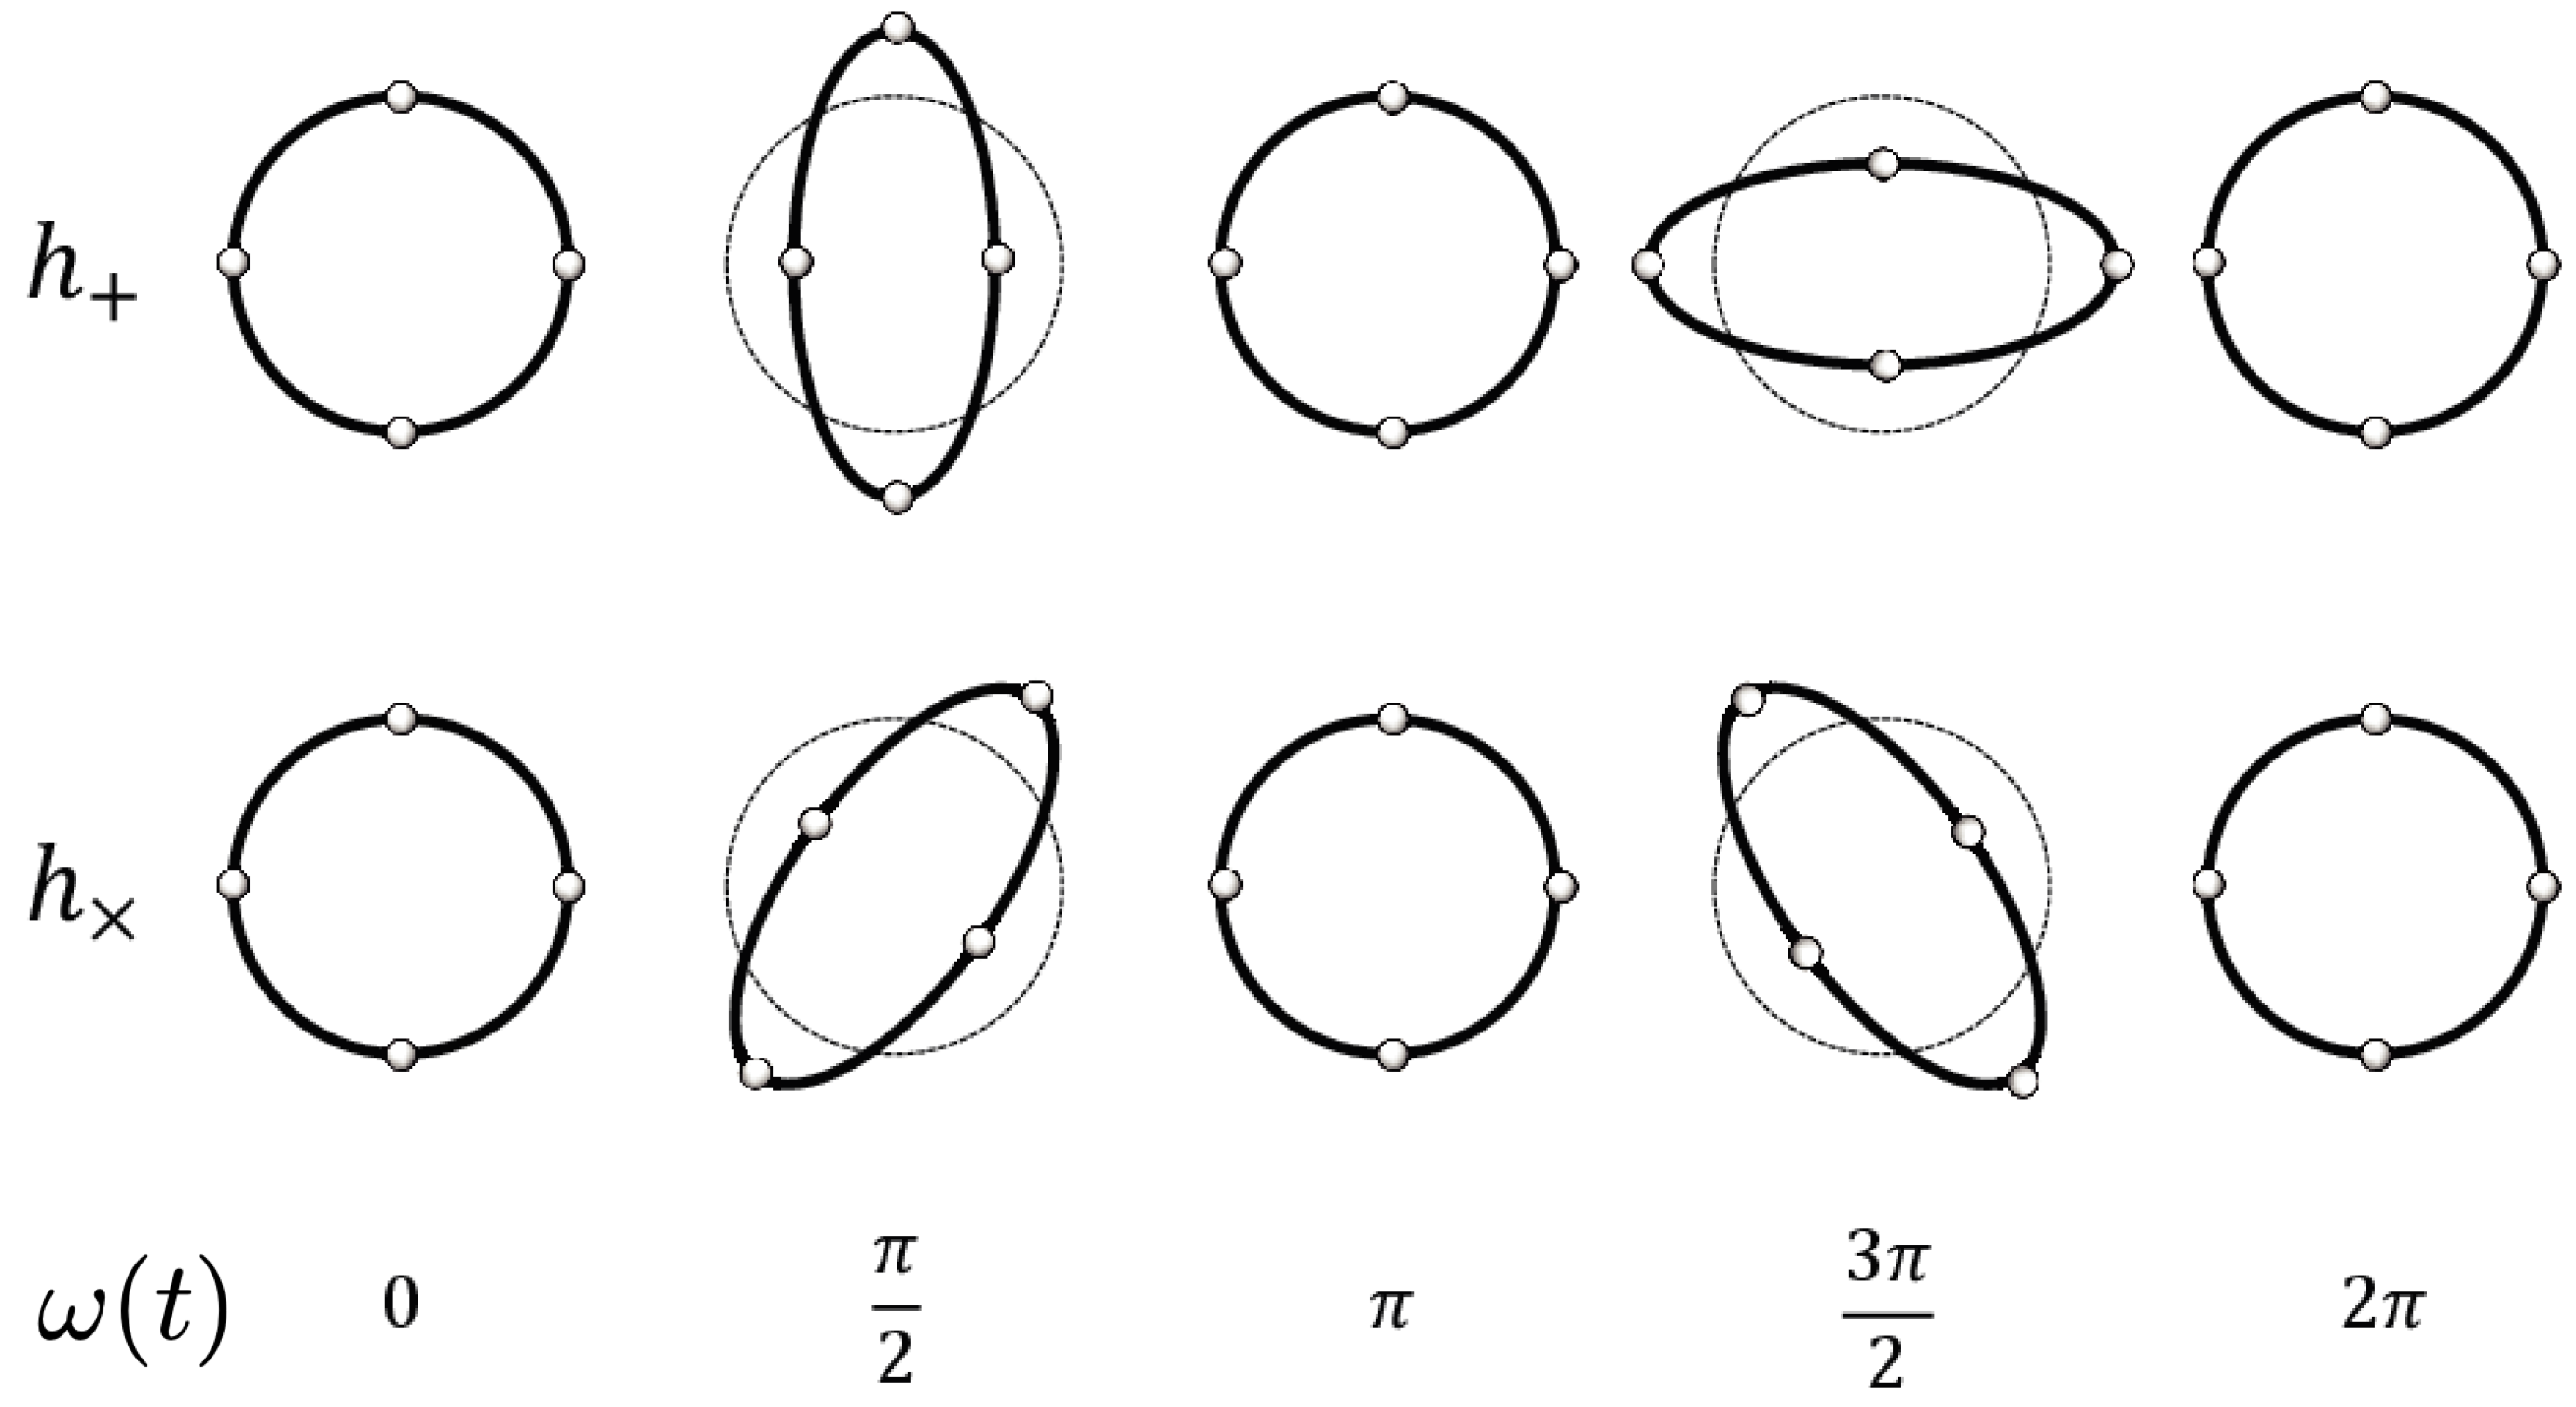
\includegraphics[scale=1]{ring}
                \centering
                \caption{The effects of plus and cross polarization on a ring of test masses.
                         The plus polarization alternately compresses and stretches the x- and y-separations.
                         The cross polarization has the same effect only rotated by  $\ang{45}$.}
                \label{fig:ring}
                \end{figure}

\section{Interferometer’s response to a gravitational wave}

        Interferometers are sensitive to the relative difference between two distances, the so-called strain \cite{6} .
        Suppose we have an interferometer with its arms pointing along the unit vectors $u^i$ and $v^i$. The strain $h(t)$ is given by
                \begin{equation}
                	h(t) = {1 \over 2} (h_{ij}u^iu^j - h_{ij}v^iv^j) = D^{ij}h_{ij}(t)
                \end{equation}
        where $D^{ij}$ is referred to as the detector tensor and is given by
                \begin{equation}
                	D^{ij} = {1\over 2} (u^iu^j -v^iv^j)
                \end{equation}
        As the expression for $h(t)$ is linear in $h_{+}$ and $h_{\times}$, one can also write
                \begin{equation}
                	h(t) = F_{+}h_{+} (t) + F_{\times}h_{\times}(t)
                \end{equation}
        where $F_{+,\times}$ are called the beam pattern functions. Suppose we have a detector
        with arms that are perpendicular to each other, one pointing in the x-direction and the other
        in the $y$-direction in a Cartesian coordinate system. This detector frame, denoted by $(x,y,z)$,
        is generally different from the GW coordinate system, denoted by $(x^\prime,y^\prime,z^\prime)$, where the source
        is conveniently described. To account for such a difference, we first note that when the plus
        and cross polarisations are not equal in strength, we can rotate the coordinate system by
        an angle $\psi$ around the $z^\prime$ axis so that the $x^\prime$ and $y^\prime$ axes
        coincide with the mayor and minor axis of the associated ellipse. \\
        In going from the GW frame to the detector frame, we can rotate the GW frame by
        an angle $\theta$ around the $x^\prime$ axis and an angle $\phi$ around the $z^\prime$ axis,
        where the angles $(\theta, \phi)$ denote the direction of propagation of the GW in the detector frame.
        Applying these three rotations, the beam pattern functions for a detector with perpendicular arms are given by
                \begin{align}
                F_{+}^{\ang{90}}& = {1 \over 2} (1 + \cos^2 \theta)\cos 2\phi \cos 2 \psi - \cos \theta \sin2\phi \sin2\psi \\
                F_{\times}^{\ang{90}}& = {1 \over 2} (1 + \cos^2 \theta)\cos 2\phi \sin 2 \psi + \cos \theta \sin2\phi \cos2\psi
                \end{align}

\subsubsection{Non-stationary transient noise sources}
	
	The various noises of the detector can be conveniently characterized by a spectral strain
        sensitivity with dimensions of $1/\sqrt{Hz}$, as we explain in this section. 
        The detector output $s(t)$ is composed of instrumental noise $n(t)$ arising from
        naturally occurring random processes and a potential strain signal $h(t)$
                \begin{equation}
                	s(t) = n(t) + h(t)
                \end{equation}
        The detection problem then becomes how to distinguish $h(t)$ from $n(t)$ when $h(t) << n(t)$.
        In a way, $n(t)$ provides a measure of how small an $h(t)$ we can detect.
        Thus we take $n(t)$ as the detector’s noise and have a convenient way to
        compare performances of different detectors.
	The instrument response $s(t)$ can be also expressed as a convolution of the antenna patterns 
	with the two GW polarizations $h_{+}, h_{\times}(t)$:
		\begin{equation}
			s(t) = n(t) +  F_{+}h_{+} (t) + F_{\times}h_{\times}(t)
		\end{equation} 
	The antenna patterns depend on the frequency and sky location of the source; 
	for wavelengths that are large compared to the detector, the antenna patterns are simple quadrupoles \cite{19}.
	The information contained in the time series is usually represented in the Fourier domain 
	as a strain amplitude spectral density, $h(f)$. \\
	This quantity is defined in terms of the power spectral density $S_s(f) = \tilde s^{*}(f) \tilde s(f)$
	of the Fourier transform of the time series:
		\begin{equation}
                	\tilde s(f) = \int^{\infty}_{-\infty} e^{-2 \pi ift} s(t)dt
		\end{equation}
	The strain amplitude spectral density is then defined as $h(f) = \sqrt{S_s(f)}$.
	Noise is categorised as either displacement noise, which directly moves the suspended mirrors
        causing a differential change in the arm cavity lengths, or as sensing noise,
        which appears in the readout signal but is not caused by a GW. \\
        We describe the principal noises that dominate the limits of our sensitivity, (Fig.$\ref{fig:noise2}$).
		\begin{figure}
                        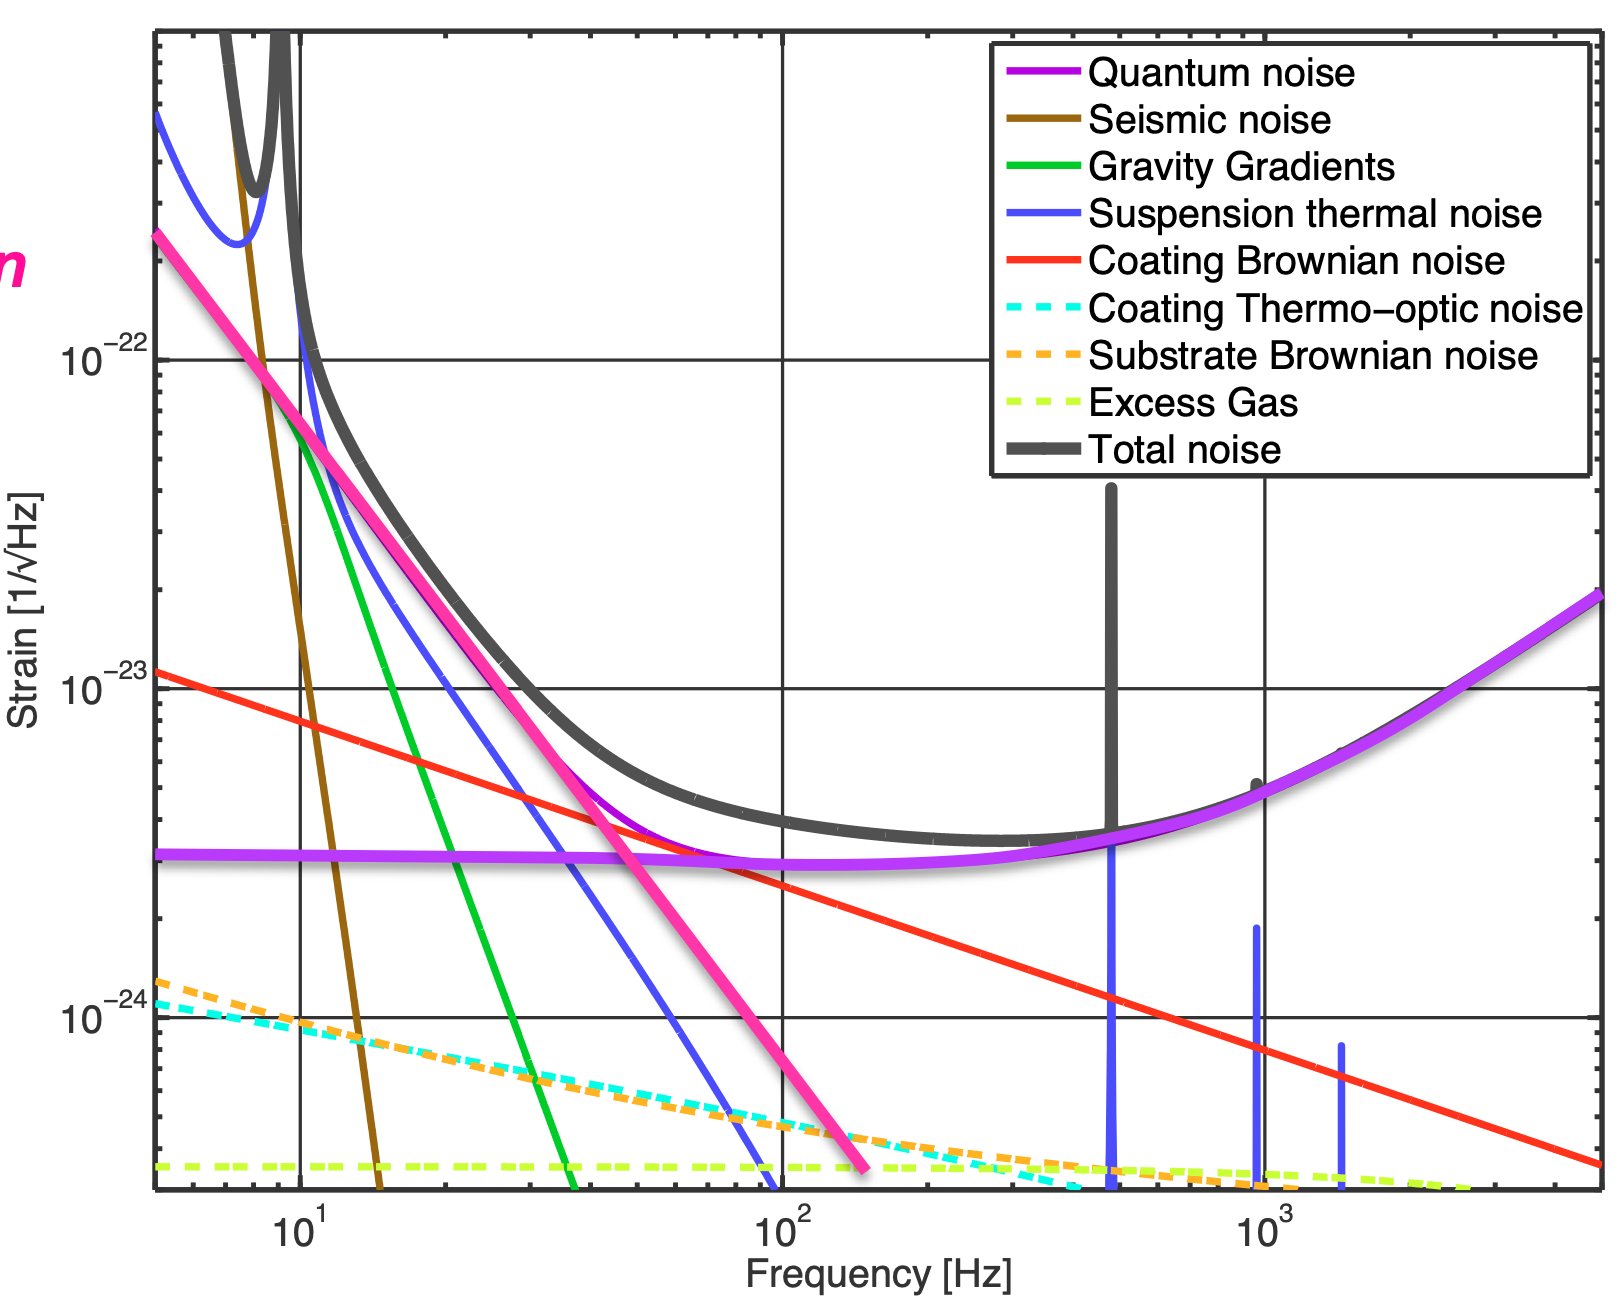
\includegraphics[scale=0.3]{noise2}
                        \centering
                        \caption{The strain equivalent spectral amplitudes $\sqrt{S_n(\omega)}$ 
				 of several noises couple to the detector. 
				 Most relevant contributions comes from quantum noise 
				 and from thermal noise of mirror coating and suspensions. 
				 Seismic noise dominates below 10Hz}
                        \label{fig:noise2}
                \end{figure}
        At lower frequencies, up to 10Hz, the main contribution to the global noise
        is due to vibrations of the ground which couple to the mirror motion, (Fig.$\ref{fig:noise2}$ brown line): 
	it shakes the optics and produces strain signals that mask GW signals. 
        This seismic noise is caused by earthquakes, weather and human activity.
        To reduce the potential movements of the optical elements,
        the mirrors are isolated using an advanced suspension system. \\
        At frequencies where the seismic motion has been sufficiently reduced,
        between 10Hz and 500Hz, the random Brownian motion of the molecules on the surface of the mirrors and wires dominates (Fig.$\ref{fig:noise2}$ red line). \\
        The thermal energy of the interferometer’s components induce vibrations both in the suspensions and in the mirrors.
        The nature of GW signal requires the sensitivity of the interferometric detectors
        to be extremely high in broad frequency band.
        Therefore, the power spectrum density of the thermal noise must be considered in the development of the detectors.
        The Fluctuation-dissipation Theorem relates the spectrum of the thermal noise to the amount of dissipation
                \begin{equation}
                	S_{n}(\omega) = - {{4k_bT} \over {\omega}} Im[H(\omega)]
                \end{equation}
        From this equation is possible to state that the energy of fluctuations has a frequency dependent distribution;
        $H(z)$ is the transfer function of the system, it is a mathematical function that models the device’s output, defined as
                \begin{equation}
                	H(x) = {1 \over {iWZ(\omega)}}
                \end{equation}
        In which $Z(\omega)$ is the impedance of the system in the frequency domain that can be computed as the ratio
        between the Fourier components of the generalised force $\tilde F(\omega)$ and the response of the system $\tilde X(\omega)$
                \begin{equation}
                	Z(\omega) = {{\tilde F(\omega)} \over {i\omega \tilde X(\omega)}}
                \end{equation}
        In the case of an harmonic oscillator, the noise spectral density is
                \begin{equation}
                	S_n(\omega) = {{4k_bT} \over {m\omega}} {{{\omega_0}^2 \phi(\omega)} \over {(\omega^2-{\omega_0}^2)^2 + {\omega_0}^4 \phi^2(\omega)}}
		\end{equation} 
	Generally, thermal noise can be reduced decreasing the dissipation with monolithic suspensions and better coatings
        other than lowering the temperature using criogenic payloads as it is done in KAGRA.
        Quantum mechanics limits the precision at which the test mass positions can be determined. \\
        At high frequencies, photon shot noise limits the sensitivity, 
	while at low frequencies it is limited by radiation pressure.
        The photon shot noise is produced by the natural fluctuations in the rate of photons arriving at the photodiode,
        that follow a Poisson process. The noise will decrease with increasing laser power,
        recycling cavity gain, arm cavity gain, and arm length.
        The corresponding noise spectral density is
		\begin{equation}
                	S_n(\omega) = \Bigg({{\lambda_{laser}} \over {4 \pi L}}\Bigg)^2 {{2 \hbar \omega_{laser}} \over {P}}
                \end{equation}
        Radiation pressure noise is associated with the photons from the laser striking the mirror
        and causing a force on the mirror. Of course, increasing the laser power to combat shot noise
        will actually result in an increase of radiation pressure.
                \begin{equation}
                	S_n(\omega) =  {{32 \hbar \omega_{laser}P} \over {(4MLc \pi^2 f^2)^2}}
                \end{equation}
        This is an example of the Heisenberg’s Uncertainty Principle, which says that the knowledge
        of the position and the momentum of a body is restricted from the relation $\Delta x \Delta p \geq \hbar$. 
        The high laser power required to determine the position of the test masses exerts
        a fluctuating radiation pressure which perturbs the test mass positions. 
        The minimun noise level is called Standard Quantum Limit (SQL) and sets a fundamental limit
        on the sensitivity of beam detectors, contributing to the noise as
                \begin{equation}
                	S_n(\omega) = {{2 \hbar} \over {M(\pi f L)^2}}
                \end{equation}
        Moreover, the presence of residual gas in the beam tubes would worsen the performance
        of the mirrors and of the laser; for this reason the vacuum system is maintained at a pressure
        of below $10^{-6}$Pa and the noise curve of the interferometer includes only
        the most dominant residual gas component, hydrogen, at a pressure of $10^{−7}$ Pa. 
		\begin{figure}
                	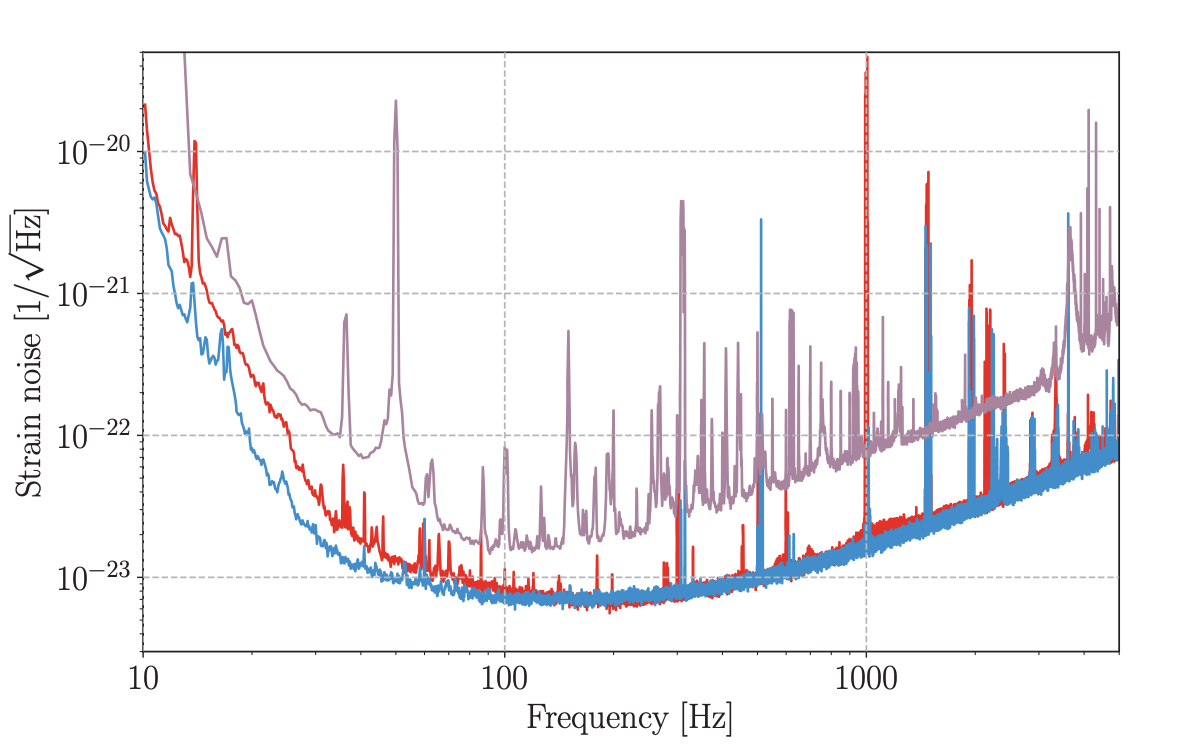
\includegraphics[scale=0.6]{noise1}
                	\centering
                	\caption{Amplitude spectral density of the total strain noise 
				 of the Virgo, LHO, and LLO detectors. 
				 The curves are representative of the best 
				 performance of each detector during O2 \cite{13}.}
                	\label{fig:noise1}
                \end{figure}

\subsection{Sources}

	There are four different classes of physical sources 
	that are potential sources of GWs 
	of sufficient amplitude to be detectable 
	by current or theorised GW detectors. 

\subsubsection{Coalescing compact binaries}

	Compact binary star systems, in which each member is a neutron star or black hole, 
	are currently the only observed sources of GWs.
	They are an ideal source for ground based GW detectors, 
	as their compactness allows their orbital separation to become 
	small enough before they merge for them to emit GWs in the detectors sensitive frequency band.
	If one of the components of the binary is a neutron star 
	then there may be an electromagnetic counterpart to the GW signal \cite{20}. 
	The loss of energy from the system will cause the orbital radius to decay, 
	the frequency to increase, and the amplitude of the radiation to increase, 
	producing a distinctive chirp-like signal. 
	Eventually, the two objects will be close enough to merge together, 
	and the new single object will pulsate in an excite state as it tries to return to equilibrium \cite{21}. 
	If the remanant is a BH, this phase is known as the ringdown phase and it is well-modeled as a series of quasi-normal modes. 
	As the form of the gravitational radiation can be predicted allows 
	a more sensitive search to be performed: knowing the form of the signal 
	that is being search for allows powerful matched filtering techniques 
	and signal consistency tests to be used in the attempt to detect such signals.


\subsubsection{Bursts}

	A burst of GWs is an event that releases a large amount 
	of gravitational energy over a very short period of time, typically less than a few seconds.  
	Astrophysical events that are believed to result in a transient signal 
	include gamma ray bursts and supernovae explosion as well as the final stages of a coalescing binary. 
	GW signal with a partially modelled or unknown waveform, 
	this may be due to unknown or complicated physics, or the source may be something totally unpredicted. 
	The matched filtering is not a useful technique to search for this type of signal, 
	as the waveform of a GW burst signal is unknown \cite{3}. 
	Searches for GW bursts typically search for excess power that occurs coherently between multiple detectors.  
	Even with no knowledge of the source of a GW signal, 
	it is still possible to estimate some of the source parameters. 
	Searches for GW bursts typically give estimations of the duration, 
	amplitude and frequency of the source. \\
	An estimation of the sky position is given by measuring the difference 
	in arrival time between different detectors. 
	If the distance to the source is known, 
	perhaps through an electromagnetic counterpart, 
	then it is possible to estimate the energy of the source. 


\subsubsection{Continuous Sources}

	A periodic source is a source that emits at constant or nearly constant frequency.
	The prototypical source of continuous GWs is high frequency rotating neutron stars 
	with a non-axial deformation or low frequency binary systems 
	composed of white dwarfs or black holes far from merger. 
	These sources should be present throughout the operational lifetime of a detector, 
	so the greater the observation time, the better the sensitivity to periodic sources becomes. 
	Spinning neutron stars will lose energy and spin down over time, 
	and this energy loss is due to a number of different mechanisms, 
	including emission of gravitational radiation \cite{3}. 
	To emit a continuous GW with characteristic amplitude, 
	a neutron star must have a non-axisymmetry in the crust. 
	The radiation amplitude is proportional to the crucial parameter $\epsilon$, 
	the fractional asymmetry that is proportional to the mass of the bump on the surface. \\
	As neutron stars emit electromagnetic radiation, 
	it is possible to target searches of GWs for neutron stars with positions, 
	frequencies and spin-downs known from X-ray, radio and gamma-ray observations. 
	Examples are the Crab and Vela pulsars. 
	Continuous GWs have not yet been detected, 
	but current searches have produced upper limits for their emission. 
	Upgraded interferometers in LIGO could set an upper limit on  
	$\epsilon$ of order $10^{-6}$ for sources at $\sim10$ kpc, 
	and explain how a neutron star can be distorted to give a value of $\epsilon$ that is interesting as a GW source. 
	Whatever the mechanism generating the distortion, 
	it is clear that  $\epsilon$ will be small,
	so that $h \sim 10^{-24}$ or smaller, which is quite weak. 
	Measuring these waves will require
	coherently tracking their signal for a large number of wave cycles, 
	which is actually quite difficult, 
	since the signal is strongly modulated by the Earth’s rotation and orbital motion.\\
	Searching for periodic GWs means demodulating the motion of the detector, 
	a computationally intensive problem since the modulation is different for every sky position \cite{4}. 
	Unless one knows in advance the position of the source, 
	one needs to search over a huge number of sky position "error boxes”.

\subsubsection{Stochastic background}

	Stochastic backgrounds are “random” GWs, 
	arising from a  number of sources that overlap 
	in time and frequency that are not individually resolvable \cite{22}. 
	The sum of the signals at any given time and frequency will have 
	a random pattern that may be analyzed statistically but not predicted precisely.
	A particularly interesting source of stochastic waves is the dynamics of the early Universe, 
	which could produce an all-sky GW background, 
	similar to the cosmic microwave background. \\ 
	However, to measure waves from this epoch, 
	we would need much more sensitive detectors than the ground-based interferometers available.
	Stochastic backgrounds are usually idealized as being stationary, 
	isotropic and homogeneous and because of their random nature they look just like noise \cite{4}.	
	Another possible background could come from astrophysical sources. \\ 
	These possible sources include a population of rotating neutron stars 
	and a population of white dwarf binaries that would be important mostly for a space-based interferometers such as LISA. 

%----------------------------------------------------------------------------------------------------------------------------------------------------------------------------------------------------------
\chapter{Data Analysis for Coalescing Binary Systems}

	The main role of data analysis in GW detection is to extract the GW signal 
	buried into noisy interferometric strain data, which can be characterised by a spectral strain sensitivity.
	The data analysis technique depends on the type of source.
	GW searches from the inspiral, merger and ringdown phases of compact binary systems 
	are based on two broad techniques: 
	modeled searches which use theoretical waveforms for such systems 
	as predicted by general relativity and 
	unmodelled or burst searches which assume minimal information about these waveforms \cite{23}. \\
	Although signals from coalescing binaries will most probably not stand above the broadband noise of the detector, 
	their detection is possible by the use of matched filtering, 
	which takes advantage of the fact that the wave form can be fairly well predicted. 
	This technique is the optimal detection strategy in Gaussian noise 
	in searching for GWs with well understood waveforms. 

\section{Matched Filtering}

	The filtering procedure involves correlating the detector output 
	with a copy of the expected waveform, 
	called a matched filter or a template.
	A real detector functions only over a finite frequency band, 
	and acquires data at a finite sample rate \cite{24}. 
	In this case, the noise power spectrum $S_n$ 
	may be taken to be infinite outside the bandwidth of the instrument, 
	effectively restricting the range of integration to lie between $[-f_N, f_N]$, 
	where $f_N$ denotes the Nyquist frequency $f_N = 1/(2\Delta t)$, 
	and $\Delta t$ is the time between successive data samples.   \\
	The measured detector’s strain amplitude, $s(t)$, may or may not contain a signal,
	thus it will be composed of $n(t)$, the real strain-equivalent noise
        produced by fluctuations within the detector and its environment, 
	and possibly a GW of known form, $h(t)$
                \begin{equation}
                        s(t) = h(t) + n(t)
                \end{equation}	
	or if there is no signal   		
		\begin{equation}
                        s(t) = n(t)
                \end{equation}
        assuming that the detector noise is well described as stationary Gaussian noise with zero mean and one-sided PSD, $S_n(f)$.
        The aim of the match filtering is to look for a filter function,
	whose output, when passing the data through this filter, 
	will be large when a signal is present and small otherwise. 
        If the waveform, $h(t)$, embedded in stationary Gaussian noise is known, 
        the optimal filter, $K(t)$, has the following form
		\begin{equation}
 			K(t) = \tilde h_{template}/S_n
		\end{equation}
	where $\tilde h_{template}$ is the waveform template to match the signal.
	The output of the filter is obtained from a weighted inner product in the frequency domain, 
	cross-correlating the data with the inverse noise power weighted data from each of the detectors:
		\begin{equation}
 			(s|h)(t) = 4Re \int^{f^{high}}_{f^{low}} {{\tilde s (f) \tilde h^{*}_{template}(f)} \over {S_n (f)}} e^{2 \pi if} 
		\end{equation}
	The frequency limits $f_{low}$ and $f_{high}$ are determined by the bandwidth of the detector’s data.
	Here $\hat s(f)$ denotes the Fourier-transformed detector data, defined by
		\begin{equation}
			\hat s(f) = \int^{\infty}_{-\infty} s(t) e^{-2i \pi tf} dt
		\end{equation}
	and $\tilde h(f)_{template}$ denotes the Fourier-transformed template waveform 
	and $S_n(f)$ is the one-sided power spectral density of the detector noise. 
  
\subsection{Signal to noise ratio}

	Finding the form of the filter which will optimally extract the signal from the noise,
        means locating the maxima of the output of the matched filter, $(s|h)$, 
	over the arrival time and phase.
        This quantity, $(s|h)$, could be used to set a threshold value such that 
	a $|(s|h)|$ above the threshold would indicate a signal
	and below would indicate no signal. \\
	However, the filter output can be normalized by the variance of the optimal filter, $\sigma^2$,
	which is an estimation of the uncertainty in a measurement of $(s|h)$, due to noise in the detector:
                \begin{equation}
                        \sigma^2 =4 \int^{\infty}_{0} {{|\tilde h_{template}(f)|^2} \over {S_n(f)}}df
                \end{equation}
 	The normalized output of the optimal filter is a new thresholding statistic and can be defined as  
	the signal to noise ratio (SNR), the ratio of the observed filter output to its,
        expected or observed, root-mean-square fluctuations \cite{24}:
                \begin{align}
                        \rho(t) &= {{| (s|h) |} \over {\sigma_{h}}} \\
                             &= {{(\tilde h_{template}|\tilde h)} \over {\sqrt{(h_{template}|h_{template})}}}
                \end{align}
        The value of the SNR will then be proportional to the amplitude of the signal buried in the noise.
	The smart choice for a threshold that can be set on this value is such that
	it can admit as many signals as possible, while still keeping the false alarm rate low. 

\subsection{Matched Filtering for Compact Binary Signals}

	An interferometric detector is sensitive to a linear combination 
	of the two GW polarizations where the GW signal has the form \cite{26}: 
                \begin{equation}
                h(t) = F_{+}h_{+} (t) + F_{\times}h_{\times}(t)
                \end{equation}
	where $F_{+}$ and $F_{\times}$ are the two antenna response functions of the detector, 
	which depend on $\theta$ and $\phi$, 
	the spherical coordinates of the sources sky position with respect to axes defined by interferometers’ arms. 
	Due to the nature of GW signals from the inspiral phase of CBCs, 
	it follows that the phase evolution of the cross polarization is $\ang{90}$ out of phase with the plus polarization, given by 
		\begin{equation}
			h_{+}(t) = A(t) cos (\phi (t))
		\end{equation}
		\begin{equation}
			h_{\times}(t) = A(t) sin (\phi (t))  
		\end{equation}
	where $A(t)$ is the amplitude evolution of the signal 
	and $\phi(t)$ is the phase evolution of the signal. 
	The Fourier transform of the two polarization are related by $\tilde h_{+} = ih_{\times}$, 
	which means that the inner product between the orthogonal polarisation is zero 
		\begin{equation}
			(h_{\times}|h_{+}) = 0
		\end{equation}
	Hence, when filtering  $s = (Xh_{+}/\sigma_{h}) + (Y h_{\times}/\sigma_{h}$ 
	with the template $h_{+}$ and $h_{\times}$, 
	respectively, we obtain the matched-filter real-time series
		\begin{equation}
			z_{+} = X\sigma_{h}
		\end{equation}
		\begin{equation}
			z_{\times} = Y \sigma_{h} 
		\end{equation}
	Which leads to the definition of the two-phase filter, 
	which has twice the degrees of freedom of a single-phase filter:
		\begin{equation}
			\rho = {1 \over \sigma_h} \sqrt{|z_{+}| ^2+ |z_{\times}|^2}
		\end{equation}
	The bonus of extracting information from both polarizations of the GW 
	comes with the cost of increasing the expectation value of $\rho$ when there is no signal present. 
	For a detector output that includes a signal at distance $D_eff$, 
	$s(t) = n(t) + (D_eff/1 Mpc)^{-1}h_{1Mpc}$, 
	a biased estimate of the effective distance for a given trigger 
	can be defined by combining the definition of the SNR with the template normalization $\sigma_h$:
		\begin{equation}
			\hat D_eff = {{\sigma_h} \over {\rho}}
		\end{equation}
	In reality, the parameters of astrophysical systems will not be known a-priori, 
	and searches must therefore be sensitive to signals at any location in the parameter space \cite{25}. 
	Performing the matched-filter calculation at every point in the full parameter space 
	would be extremely computationally prohibitive, 
	and therefore a number of analytic approximations are used to reduce the size of the parameter space. 
	It is assumed that the “extrinsic” parameters of a GW signal, 
	such as the sky-location, source orientation, polarisation phase and distance, 
	can all be absorbed by applying a constant phase-shift, 
	constant time-shift and a constant amplitude scaling to the observed waveform \cite{27}. 
	With these assumptions in place, 
	one can analytically maximise over an overall amplitude and phase of the signal, 
	and use an inverse Fourier transform to quickly evaluate the statistic as a function of time. \\
	The component masses and spins, 
	which are the only intrinsic parameters, 
	are searched over by repeating the search process with a well chosen discrete set of waveform models 
	with varying values of the component masses and spins, 
	known as the template bank \cite{27}. 
	Physically, these assumptions hold if one assumes that the sources being observed 
	have no orbital eccentricity, no precession and no contribution from higher-order modes 
	to the gravitational-wave signal \cite{23}. 

\section{Template Bank}

	To perform a matched-filtered search that would recover any compact binary system 	
	with minimal loss in SNR over a given range of intrinsic parameters 
	one must filter the data against a a bank of templates, 
	to obtain an estimation of the parameters for the source of the signal 
	from the template that provided the largest SNR.
	The manifold of waveforms is a continuous space in the component masses, 
	of which we are only able to search discrete points, 
	which have to be placed in such a way that any signal
	that has parameters in the space will still produce an SNR 
	above threshold by matching with the “closest” template. 
	In order to compute the distance between two templates of different parameters, 
	one can create a metric over the parameter space and then compute the the error between the two waveforms.
	Two neighbouring templates can be defined as $\hat h(f;\lambda)$ and $\hat h(f;\lambda + \Delta \lambda)$,
	where $\lambda = \{\lambda_{intr}, \lambda_{extr}\}$ is the a set of 
	the intrinsic (masses and spins) and extrinsic parameters (time of arrival and phase).
	Using the overlap of two waveforms, defined as the inner product inversely weighted 
	by the one-sided PSD $S_n(f)$ of the detector noise, one can compute the match:

		\begin{equation}
			\mathcal{M}(\lambda, \Delta \lambda) \equiv max_{\Delta \lambda_{extr}} \langle\hat h(f;\lambda), \hat h(f;\lambda + \Delta \lambda)  \rangle
		\end{equation}

	The match is maximised only over the extrinsic parameters, 
	because waveforms related by time and phase offsets
	are described by the same template, 
	since all possible coalescence times and phases are searched for.
	This expression can be Taylor-expanded about $\Delta \lambda = 0$:

		\begin{equation}
			\mathcal{M}(\lambda, \Delta \lambda) \simeq 1 - g_{ij} \Delta \lambda^i \Delta \lambda^j
		\end{equation}

	Where 

		\begin{equation}
			 g_{ij} \equiv -{1 \over 2} ({{\partial^2\mathcal{M}} \over {\partial  \Delta \lambda^i  \partial. \Delta \lambda^j}})_{\Delta \lambda = 0}
		\end{equation}

	can be interpreted as a metric in the parameter space, which is also defined
	by the mismatch $MM = (1 − \mathcal{M})$ between two templates.
	Any mismatch between signal and template leads to a loss in SNR, 
	and down-weighting by the signal-based vetoes. 
	When constructing a template bank, this mismatch can be also interpreted 
	as the proper distance in the parameter space,	

		\begin{equation}
			ds_{ij}^2 = 1 − \mathcal{M} = g_{ij} \Delta \lambda^i \Delta \lambda^j
		\end{equation}

	which should be chosen so that the loss in signal-to-noise ratio due to the mismatch 
	of the template with the signal does not deprecate the detectability of these sources.

\subsubsection{Fitting factor}

	The standard measure for deciding what class 
	of waveforms is good enough is the fitting factor, $FF$.
	The fitting factor i quantitatively describe closeness of 
	the true signals to the template manifold, in terms of the fraction of 
	signal-to-noise-ratio obtained when filtering 
	the data with an approximate family of templates. 
	To quantify the bank coverage, usually Monte-Carlo simulations carried out   
	to compute the distribution of fitting factors of the banks against 
	a set of injected signal waveforms with randomly chosen parameters. 
	The fitting factor, $FF$, of a template bank with respect to an injected signal $h_{*}$ 
	is defined as the maximum value of match over all the templates:

		\begin{equation}
			FF(h_{*}) = max \mathcal{M}(\hat h_{*}, \hat h(\Lambda))
		\end{equation}

	assuming that the signal model is the same for both templates and injections. 
	The fractional loss of SNR in capturing the signal 
	$h_{*}$ with the template bank is $1 - FF(h_{*})$.

	If the fitting factor is less than unity, the signal lies outside the parameter space, 
	and the fitting factor represents the cross-correlation between 
	the signal and the template nearest it in parameter space. 
	This loss arises from the discrete placement of the templates. 
	Because binaries are, on large scales, uniformly distributed in space 
	and because the signal strength scales inversely with distance, 
	the fraction of event rate retained is approximately FF. 
	Therefore it is desirable that the template bank is constructed such that 
	no putative signal anywhere in the parameter space
	has a FF value less than the minimal match. 
	A bank is said to be effectual if it can satisfy this condition.
	It has become conventional to regard $FF = 97\%$, 
	which translates in $10\%$ loss of event rate, as a reasonable goal.


\subsubsection{Frequency bound}

	An algorithm that most efficiently covers the parameter space relies on the choice of a coordinate system, 
	in which the metric is as flat as possible across the space.
	In computations with the two-mass-parameter waveforms, 
	the best coordinates to use on the parameter space are not the two masses, 
	but rather the inspiral times, chirp times, from some fiducial frequency to final merger, 
	as computed at Newtonian and first post-Newtonian order. 
	The metric components are slowly varying over the parameter space, 
	when expressed in as dimensionless chirp times.
	

        The lower frequency cutoff $f_L$, which essentially determines the size of the parameter space
        of chirptimes and plays a crucial role in the computational resources required
        to process the data through the template bank.
        The initial fiducial frequency $f_L$ defines the range of values of the chirptimes
        and is not itself a parameter to search for.
        However, it affects the length of the signals
        (therefore, the parameter space to be covered) and the SNR extracted.

\subsection{Template placement}


	The computational cost of any GW search
	 is directly proportional to the number of templates used.
	It is therefore vital to have a method that enables one 
	to place a template bank using as few templates as possible. 
	Two broad classes of template-placement algorithms 
	have been developed in the literature. 

\subsubsection{Stochastic placement}

	Stochastic methods place templates, 
	that are randomly drawn from an initially chosen distribution, 
	at random points in the parameter space.
	The bank is gradually built by comparing the newly drawn waveform
	with previously accepted templates, 
	and keeping only the ones that are sufficiently far away 
	from the ones the bank already has.
 	Those that are too similar to at least one existing waveform are discarded.
	This procedure continues until the pre-set convergence threshold is reached, 
	resulting in a final saturated template bank.
	The threshold is measured from the the ratio of rejected templates over the total number of template candidates.
	Stochastic placement, however, has the shortcoming that 
	a large number of trial waveforms needs to be drawn before convergence is achieved 
	(much more than the required number of templates in the bank). 
	This method also tends to over-cover the parameter space, 
	in the sense that the average template density is higher than optimal at fixed minimum match.
	Furthermore, the construction of a stochastic template bank 
	can be computationally demanding since, in principle, 
	each new proposed template needs to be compared 
	with previously chosen templates. 
	This problem becomes particularly acute 
	the closer the bank gets to saturation. 
	The computational problem also becomes especially demanding 
	when precession effects are considered as these additional degrees 
	of freedom require a large number of templates. 
	It is therefore important to consider methods of optimising a template bank, 
	specifically finding ways of improving effectualness for a given number 
	of templates and reducing the computational cost. 

\subsubsection{Geometric placement}


	A different method to construct the bank is geometric placement:
	this means building a flat, linear space in such a way that embeds the space of physical waveforms. 
	Hence, a crucial point is to identify a set of coordinates 
	in which the parameter space metric is almost constant: 
	the Euclidean distance in this space coincides with the matched-filtering overlap 
	between waveforms, making these coordinates naturally suited to define a regular lattice. 
	The minimal match determines the choice of spacing of the discrete template parameters 
	and therefore the number of discrete templates in the family.
	The most significant drawback of such banks is the amount of fine-tuning required 
	in order to cover “holes” across local patches because of the misalignment 
	of the cells arising from the variation of the metric. 

\subsubsection{Hybrid placement}

	In practice, a combination of the two methods is often a better strategy. 
	For example, one can place templates geometrically at low masses 
	and stochastically at high masses, or one can use many small patches 
	with regularly spaced templates, which are themselves placed stochastically 
	to cover the entire parameter space. 

\subsubsection{Compact Binary Spin}

	An observed GW signal from compact  binary coalescence, CBC, is a powerful tool, 
	that can be used to estimate the parameters of the merging binary,
	which can then provide information about the formation processes of the system. 
	However, the processes which lead to compact binary formation  
	depend sensitively on a number of poorly constrained parameters, 
	such as the typical stellar metallicity at formation, 
	the distribution of supernova kicks, 
	and the binding energy of the common envelope. 
	There are two main channel through which compact objects can be formed:
	the coevolution of two massive stars in a binary and 
	the dynamical capture of two preformed compact objects 
	in dense stellar environments such as globular clusters.
	
	In particular, it is thought that compact binaries formed by dynamical capture 
	are more likely to have component spins
	at large angles to the orbital angular momentum, 
	while those formed by common evolution are more likely to have 
	spins that are nearly aligned with the orbital angular momentum.
	Present observations clearly indicate the potential for large spins 
	on black holes in binaries, possibly close to the Kerr limit $|S/m^2| = |\chi| = 1$.
	Very few measurements of the angles between the spins and 
	the orbital angular momentum exist from electromagnetic observations. 
	In some cases, one can measure this spin misalignment via GW emission, 
	as misalignment leads to precession of the orbital plane, 
	which appears as phase and amplitude modulations in the observed signal.

	Almost all searches for GWs from coalescing compact binaries 
	using the data of first generation interferometers 
	have used templates that neglect the spins of the compact objects.
	This was primarily motivated by the sensitivity of the Initial LIGO detectors:
	because the sensitivity band started above 40 Hz, 
	including spin effects greatly increased the number of templates to be searched over, 
	and the search performed, on average, no better than non spinning searches, 	
	as the increased degrees of freedom in the signal space picked up extra noise, 	
	increasing the false alarm rate. 
	However, the Advanced LIGO detectors are sensitive to frequencies above 10–20 Hz, 
	therefore detectors are able to observe the inspiral from much larger orbital separations, 
	resulting is significantly longer observed GW signal. 
	Proper consideration of the spin effects is essential in the advanced detector era, 
	as there might be astrophysical systems that are entirely missed by non-precessing searches.
	Neglecting the spin effects can cause a much larger dephasing of the template with the signal, 
	and hence considerable loss of SNR.

	Currently, waveform models with spins aligned (or antialigned) with the orbital angular momentum 
	are being used in searches with Advanced LIGO, 
	having been demonstrated that aligned-spin templates pull in more signal than noise. 
	While building a template bank with the geometric approach for these cases is feasible, 
	since a closed-form expression of the template-space metric can be computed, 
	this is not possible for binaries with generic spins. 
	This is due to the fact that, 
	if the spins are misaligned with the orbital angular momentum of the binary, 
	the spin-orbit and spin-spin interactions will cause the spins 
	(and hence the orbit also) to precess. 
	The resulting dynamics as well as the GW forms are rather complex, 
	and the modelling requires solving a set of coupled ordinary differential equations. 
	The template placement is further complicated by the large dimensionality of the parameter space 
	(two mass parameters, five spin parameters, and two angles describing the orientation of the binary, in general). 
	Detecting highly precessing systems offers a better chance to 
	disentangle the various parameters that describe the source,  
	breaking degeneracies that exist between physical parameters 
	in the emitted gravitational-wave signal.  
	This could allow a better understanding of the nature and origin of these systems.
	Although the effect of precession on the GW signal is not fully captured 
	by aligned-spin templates, it has been demonstrated that non-precessing templates 
	are also effectual in detecting binaries with generic spins if the mass ratio is moderate 
	$(m_2/m_1 \leq 10)$; these spin effects can be also described by 
	a single reduced-spin parameter in an approximate way, 
	which makes the parameter space three-dimensional, 
	using the two masses and reduced-spin as variables. 
	
\section{Candidate ranking statistic}
	
\subsection{$\chi^2$ test}

	Since the detector’s calibrated strain data contains both stationary, Gaussian noise 
	and non-Gaussian noise transients of instrumental and environmental origin,
	matched filtering does not suffice as a detection statistic.
 	Consistency checks are needed to distinguish to mitigate the effect of the noise transients,
	that can sometimes mimic the signal from a true signal,
	and to assign an accurate statistical significance to candidate signals.
  	To eliminate the worst periods of detector performance, 
	data quality investigations are conducted by looking only at the detector behaviour,  
	which is analysed by monitoring channels.
	After removing data that is not suitable for astrophysical searches, 
	noise transients, glitches, of unknown origin could still be present in the data 
	and can cause certain templates to produce high SNR values.
	To mitigate the effect of glitches, a gating procedure is applied:
	after identification of times impacting on the sensitivity of the search,
	the data are zeroed out around these times.
	Filtering the data with template banks generates a matched-filter SNR for each template in each detector;
	GPS times of local maxima that exceed the SNR threshold are recorded as triggers. 
	Waveform consistency tests are needed to determine if the morphology 
	of a candidate signal is consistent with the expectation from the triggering template waveform.
	For signals from compact binary mergers, one can construct $\chi^2$-test:
	the template is split into p non-overlapping frequency bins; 
	these bins are constructed so that each contributes equally t
	o the SNR of a perfectly matching signal. 
	The $\chi^2$ statistic compares the expected to the measured template in each bin according to 

		\begin{equation}
			\chi^2_r = {1 \over {2p-2}}   \sum_{I=1}^{I=p} || \langle   s|h_i  \rangle -   \langle  h_i|h_i   \rangle ||^2
		\end{equation}

	where $\chi^2_r = \chi^2/(2p-2)$ is the reduced chi-squared and for real GW signals this value should be near unity, 
	meaning that the data is describing Gaussian noise with an embedded signal.
	In order to combine the SNR with the $\chi^2$ test to produce a ranking statistic 
	and down-weight triggers caused by noise transients, 	
	the matched-filter SNR is re-weighted 

		\begin{equation}
		\begin{cases}
			\hat \rho &= \rho \hspace*{4.5cm}  \text{for} \hspace*{0.15cm}\chi^2_r <= 1 \\
			\hat \rho &= \rho[{1 \over 2} (1 + (\chi^2_r)^3)]^{-1/6}  \hspace*{1.5cm}  \text{for} \hspace*{0.15cm} \chi^2_r > 1
		\end{cases}
		\end{equation}

	The search requires that gravitational-wave signals be identified via matched filtering 
	in at least two independent detectors with consistent parameters. 
	To be considered a candidate event, arrival times of the GWs at each detector 
	must differ by no more than the the maximum time-of-flight between the detectors, 
	with an additional window to account for uncertainty in the measurement of the time of arrival.
 
\subsection{False Alarm Rate}

	After mitigating the effects of noise transients, the probability of remaining transients 
	occurring simultaneously in two detectors and producing a large joint 
	ranking statistic value becomes extremely small.
	In order to keep only the most representative trigger among all the triggers produced by a single inspiral signal or glitch, 
	a final clustering step is performed on coincident triggers, 
	by selecting those with the largest value of $\hat \rho$ 
	in each time window of $10s$. 
	Any other events in the same time window are discarded. 
	This ensures that a loud signal or transient noise artifact gives rise to at most one candidate event.
	In order to assess the actual significance of a candidate, 
	we need to measure the false-alarm rate, (FAR), of the search as a function of the detection statistic.
	Typically, a detector’s background FAR can be determined 
	simply by turning off the source or changing the orientation of the detector. 
  	However, since it is not possible to isolate the detectors from GWs, 
	it is impossible to directly measure the detector noise in the absence of signals.
 	To estimate the FARs the data stream is shifted in time, 
	choosing the minimum time-shift offset to be larger than the time-coincidence window 
	used to determine if signals are observed with consistent parameters in the network.
	The resulting “time-shifted” coincidences are then treated as a background noise sample. 
	This is done numerous times with different time shifts in order to obtain 
	a probability distribution for the joint detector ranking statistics. 
	Each coincident trigger is assigned a FAR given by the number 
	of background triggers, $n_b(\hat \rho)$, with an equal or larger ranking statistic, 
	divided by the total time searched for time-shifted coincidences $T_b$
		
		\begin{equation}
			FAR = {{1 + n_(\hat \rho)} \over {T_b}}
		\end{equation}

	To account for the noise background varying across the target signal space, 
	candidate and background events are divided into different search classes based on template length. 
	The significance of candidate events is measured against the background from the same class. 
	For each candidate event, one can compute the probability of finding one or more 
	noise background events in the observation time with a detection-statistic value above that of the candidate event, given by 

		\begin{equation}
			FAP(\hat \rho) \equiv P(\geq 1 \hspace*{0.1cm}\text{noise event above}\hspace*{0.1cm} \hat \rho|T,T_b) = 1 - e^{-T{{1+n_b(\hat \rho)} \over{T_b}}}
		\end{equation}

	where T is the observation time of the search.
	If a candidate event’s detection-statistic value is larger 
	than that of any noise background event, 
	then the analysis places an upper bound on the candidate’s false alarm probability. 
	The inverse of FAR specifies the waiting time before such an event from noise is seen, and it is given by 

		\begin{equation}
			IFAR = {1 \over {FAR}}
		\end{equation}   

\section{Coincident and coherent research}

	There are two main detection strategies to search for GWs 	
	from a network of detectors: coincident and coherent.

\subsection{Coincident analysis}

	A coincidence analysis searches the data from individual detectors independently 	
	and matches the candidate event lists of individual detectors for consistency,
	in the mass and time parameters of a GW signal.
	This methodology ignores the phase information at the expense of some loss in sensitivity, 
	so there is no guarantee that the observed signals in each detector 
	are compatible with a GW source with two polarisations.
	The benefit of the coincidence search is that it is not computationally expensive: 
	the dominant cost of the search is in performing a matched filter 
	of the data against a bank of template waveforms, (as seen in Section.) :
        this task is done once per detector per template.
	A search over the sky location of the signal is then trivially done 
	by time-shifting the results from the different detectors accordingly.
        Similarly, the noise background is estimated by applying larger time shifts to the data,
        significantly longer than the light travel time between detectors, to search for noise coincidences.
        In a coincidence search, it is necessary to place a threshold on the SNR of events
        which will be stored by the analysis prior to identifying coincidences.
        This means that the power in the GW signal will only be accumulated
	in those detectors where there was an event above threshold.

\subsection{Coherent}

	A coherent search is a very sensitive way to search for GWs from a network of detectors:
	this strategy treats the detectors as if they are isolated 
	and then combines the data from all detectors phase coherently, 
	appropriately correcting for time-delays and polarization phases, 
	to obtain an individual detection statistic which is then compared with a single threshold. 
	The aim of this type of search is to obtain a single statistic for the full 
	network, that is optimized in the maximum likelihood sense, 
	to effectively construct a single, more sensitive detector.
 	While this method has been applied to searches for unmodelled burst sources,
        it has proven more difficult to use for the binary merger search.

\subsubsection{Coherent SNR}
	
	The GW signal seen by detector $X$ is a combination of 
	the two polarisations weighted by the detector antenna 
	response

		\begin{equation}
			h^X(t) = F_{+}^X h_{+}(t^X) + F_{\times}^X h_{\times}(t^X) 
		\end{equation}

	where the time of arrival in detector $X$ depends upon the sky location 
	of the source relative to the detector and the time of arrival at a fiducial location, 
	for example the Earth’s centre [24]. 
	For a network of detectors, the multi-detector matched-filter
	 is defined as the sum of the single detector inner products
 
		\begin{equation}
			(a|b) \equiv \sum^D_{X=1} (a^X|b^X)
		\end{equation}
	
	where D is the number of detectors in the network. The multi-detector log-likelihood is then calculated as

		\begin{equation}
			ln \lambda = (s|h) - {1 \over 2} (h|h)
		\end{equation}

	The larger the value of $ln \lambda$, the more likely that a signal is present.
	The coherent SNR is obtained by maximising the log-likelihood 
	over the values of the waveform amplitudes:

		\begin{equation}
			\rho^2 _{coh}\equiv 2 ln \lambda |_{MAX}
		\end{equation}
 	
	In the absence of a signal, the $\rho^2_{coh}$ follows a $\chi^2$ distribution.

        While in a coincidence search requires a signal to be observed in two or more detectors, 
	resulting in the coincident SNR to be simply the sum of all power consistent with the template waveform in each detector,
	the coherent search naturally incorporates the SNR from all operational detectors.
	
	It has been demonstrated that for a signal in the absence of noise the coincident and coherent SNRs are identical. 
	For noise events, the coincident SNR includes all of the noise, 
	while the coherent SNR, incorporating only those contributions which are compatible 
	with a coherent signal at all detectors, obtains precisely the same signal but reduces the noise background. 
	
	 Even though the coherent method is highly effective at removing background noise,  
	signal consistency tests are still required to distinguish glitches from GW signals. 

\subsubsection{Null Stream Consistency}

	In the coherent analysis the data from all detectors 
	is combined to extract the two physical GW polarisations, 
	and uses this to restrict the signal model to 
	only two independent polarizations, 
	thus it is easier to distinguish transients from GW signals, 
	as those transients which do not contribute power to the signal space, and to reject incoherent background noise. 
	

	and consequently the search is more sensitive as the number of detectors in the global network increases.

        When there are more than two detectors, 
	it is possible to construct one or more null data streams 
	which contain only noise, and define the null SNR as

		\begin{equation}
			\rho^2_N = \rho^2_{coinc} - \rho^2_{coh} 
		\end{equation}

	 
	Requiring a small null SNR is an effective method to separate 
	an incoherent noise transient from a real GW signals: 
	in fact such noise events may give a large coherent SNR,
	 but it is likely to also give a large null SNR.       

\section{Injections}

	In order to test the sensitivity of a search pipeline to detect CBC signals, 
	simulated gravitational waveforms, injections, can be added o the data before filtering.
	Then a search can be performed over the data with the added injections just as it would normally do with the real data;
	by determining FARs for the injections that we recover, 	
	and noting which injections are not recovered at all,
	we can understand how well we detect certain types of sources.
	Studies of injection recovery also aid with tuning different parameters 
	of the search pipeline and setting upper limits on the rates of particular sources. 
	One method of determining sensitivity to particular injections is the efficiency, 
	or fraction of found injections, as a function of injected physical distance. 
	Another method of determining a search’s sensitivity to a particular source 
	is to examine the injected distance as a function of frequency 
	(or total mass) for missed and found injections. 
	
	These simulations can be performed in two ways: software and hardware injections.
	The former are used to verify the results obtained from software injections, 
	the latter are used for high-statistics evaluation of the performance of analyses. 

\subsection{Software injections}

	Software injections are a streaming time series of simulated gravitational waveforms, 
	generated in the software, from a synthetic population of a certain type of source, 
	described by astrophysical parameters, including the strain amplitude, sky location, 	
	and initial frequency, and added to the data stream. 
	This can be done many times, by specifying a time-step at which to place injections, 
	without disturbing the detector or significantly reducing the duty cycle of the detectors. 
	To randomize the placement, a time interval needs to be provided around 
	each time-step in which the injection is actually placed. 
	Furthermore, one can choose to set up multiple injection searches with different injection sets. 
	Thus, we can study the recovery of thousands of injections to decide on the best tuning for a search. 
	However, there is no limit to the number of software injections that can be performed. 
	The analysis of the same data can simply be repeated with different software injections present as often as is desired. 
	For the CBC low mass analysis, the process is to use software injections to tune the pipeline; 
	they are also used when calculating upper limits.
	Software injections do not offer as comprehensive a test of the infrastructure as hardware injections. 
	
\subsection{Hardware injections}

	In contrast hardware injections are performed by physically displacing
	the detectors’ test masses to simulate the response of a GW passage. 
	Even though the detectors’ response to a true GW signal is not 
	exactly the same as the response from the injection,
	the difference is well understood and it is only relevant at high frequencies.
	These hardware injections offer a better test of the sensitivity of the infrastructure than the software ones:
	they provide an end-to-end check for the search,
	from the GW being incident on 
	the detector through to making a detection, and parameter estimation analysis to recover signals in the detectors’ data. 
	The recovery of hardware injections provides an additional check 
	of the sign of the calibration between the Advanced LIGO detectors 
	using astrophysical waveforms and the recovery measures 
	the time delay of the signal in the controls system. 
	However, as hardware injections cannot be removed from the data, 
	times when hardware injections are made cannot be analysed 
	for any other signals that might be in the data. 
	Therefore, only a limited number of hardware injections can be made in a given stretch of data. 

	If a detection candidate is a true GW, 
	we should be able to reproduce the morphology of the posterior distributions 
	using the hardware injections as well as with software injection. 
	Conversely any significant differences have the potential to highlight 
	discrepancies between the observation and our waveform models, or errors in our data analysis. 
%----------------------------------------------------------------------------------------------------------------------------------------------------------------------------------------------------------
\chapter{Gravitational wave observation so far}

\section{O1}

\section{O2}

\subsection{Gamma Ray Burst}

\section{O3a}
%----------------------------------------------------------------------------------------------------------------------------------------------------------------------------------------------------------
\chapter{Black hole-neutron star binaries}



\section{Evolution of Black Hole-Neutron Star mergers}



\subsection{Tidal disruption model}




\section{Electromagnetic Counterpart of a Black Hole-Neutron Star Binary Merger}


%----------------------------------------------------------------------------------------------------------------------------------------------------------------------------------------------------------
\chapter{My contribution to gravitational dave data analysis during O3}

\section{Bank Tests}

\section{O3 offline pyGRB analysis}

\subsection{GRB190425089}

\subsection{GRB190627A}

\subsection{GRB190728271}

\section{PyCBC O3 HL C00 data preliminary runs}

\subsection{Chunk 29}

%--------------------------------------------------------
\chapter{Conclusions}

\backmatter
\cleardoublepage

\phantomsection % Give this command only if hyperref is loaded \addcontentsline{toc}{chapter}{\bibname}

\begin{thebibliography}{1}

	\bibitem{1} Albert Einstein. On the General Theory of Relativity. Sitzungsber. Preuss. Akad. Wiss. Berlin (Math. Phys.), 1915:778–786, 1915. [Addendum: Sitzungsber. Preuss. Akad. Wiss. Berlin (Math. Phys.)1915,799(1915)]. 
	\bibitem{2} Albert Einstein. Naherungsweise integration der feldgleichungen der gravitation. Sitzungsberichte der Koniglich Preu{\ss}ischen Akademie der Wissenschaften (Berlin), 1:688–696, 1916. 
	\bibitem{3} M. Maggiore. Gravitational Waves: Volume 1: Theory and Experiments. Oxford University Press, 2008
	\bibitem{4} E. E. Flanagan and S.A .Hughes. The basics of gravitational wave theory. arXiv:gr-qc/0501041v3
	\bibitem{5}  M. Blau, “Lecture Notes on General Relativity,” ICTP (2000). 
	\bibitem{6} Tjonnie G. F. Li. A. Extracting Physics from Gravitational Waves: Testing the Strong-field Dynamics of General Relativity and Inferring the Large-scale Structure of the Universe. Springer, 3 lug 2015	
	\bibitem{7} J. Weber. Detection and generation of gravitational waves. Phys. Rev., 117: 306–313, Jan 1960. doi:10.1103/PhysRev.117.306. 
	\bibitem{8} Gertsenshtein M.E.; Pustovoit V.I. On the detection of low frequency gravitational waves. Sov. J. Exp. Theor. Phys. 1962, 43, 605–607. 
	\bibitem{9} Yu, Haocun and others. Quantum correlations between the light and kilogram-mass mirrors of LIGO. [arXiv:2002.01519 [quant-ph]].
	\bibitem{10} Weinstein, A. Advanced LIGO optical configuration and prototyping effort. Class. Quantum Grav. 19, 1575–1584 (2002).
	\bibitem{11} D. G. Blair, E. J. Howell, L. Ju, C. Zhao. Advanced Gravitational Wave Detectors. Cambridge University Press, 16 feb 2012 
	\bibitem{12} Stephen Fairhurst. Triangulation of gravitational wave sources with a network of detectors. arXiv:0908.2356v2 [gr-qc]
	\bibitem{13} The LIGO Scientific Collaboration, the Virgo Collaboration. GWTC-1: A Gravitational-Wave Transient Catalog of Compact Binary Mergers Observed by LIGO and Virgo during the First and Second Observing Runs.arXiv:1811.12907v3 [astro-ph.HE]
	\bibitem{14} The LIGO Scientific Collaboration, the Virgo Collaboration. GW150914: First results from the search for binary black hole coalescence with Advanced LIGO. arXiv:1602.03839v3 [gr-qc]
        \bibitem{15} B.P. Abbott et al. (LIGO Scientific Collaboration and Virgo Collaboration). GW170817: Observation of Gravitational Waves from a Binary Neutron Star Inspiral. Phys. Rev. Lett. 119, 161101.	
	\bibitem{16} Charles W. Misner, Kip S. Thorne, and John Archibald Wheeler. Gravitation. W. H. Freeman, 1973
	\bibitem{17} Sean M. Carroll. Lecture Notes on General Relativity. arXiv:gr-qc/9712019v1
	\bibitem{18} B.S. Sathyaprakash, B.F. Schutz. Physics, Astrophysics and Cosmology with Gravitational Waves. arXiv:0903.0338v1 [gr-qc]
	\bibitem{19} Schutz, B. F. and Tinto, M. Antenna patterns of interferometric detectors of gravitational waves. I - Linearly polarized (ISSN 0035-8711), vol. 224, Jan. 1, 1987, p. 131-154.
	\bibitem{20} Francesco Zappa, Sebastiano Bernuzzi, Francesco Pannarale, Michela Mapelli, and Nicola Giacobbo. Black-Hole Remnants from Black-Hole–Neutron-Star Mergers. Phys. Rev. Lett. 123, 041102. 
	\bibitem{21} The LIGO Scientific Collaboration, the Virgo Collaboration. The basic physics of the binary black hole merger GW150914. arXiv:1608.01940v4 [gr-qc].
	\bibitem{22} C. J. Moore, R. H. Cole and C. P. L. Berry. Gravitational-wave sensitivity curves. Classical and Quantum Gravity, Volume 32, Number 1
	\bibitem{23} The LIGO Scientific Collaboration and the Virgo Collaboration. Tests of General Relativity with the Binary Black Hole Signals from the LIGO-Virgo Catalog GWTC-1. arXiv:1903.04467v3 [gr-qc].
	\bibitem{24} Bruce Allen. A chi-squared time–frequency discriminator for gravitational wave detection. Phys. Rev. D 71, 062001 (2005).
  	\bibitem{25} Collin Capano, Ian Harry, Stephen Privitera, and Alessandra Buonanno. Implementing a search for gravitational waves from non-precessing, spinning binary black holes. arXiv:1602.03509.
  	\bibitem{26} L. Wen et al 2008. Geometrical expression of the angular resolution of a network of gravitational-wave detectors and improved localization methods. J. Phys.: Conf. Ser. 122 012038.
	\bibitem{27} I. Harry, J. Calderon Bustillo, and A. Nitz, (2017). Searching for the full symphony of black hole binary mergers. arXiv:1709.09181 [gr-qc]. 

\end{thebibliography}

\printbibliography
\end{document} 

